% Template for PLoS
% Version 3.3 June 2016
%
% % % % % % % % % % % % % % % % % % % % % %
%
% -- IMPORTANT NOTE
%
% This template contains comments intended 
% to minimize problems and delays during our production 
% process. Please follow the template instructions
% whenever possible.
%
% % % % % % % % % % % % % % % % % % % % % % % 
%
% Once your paper is accepted for publication, 
% PLEASE REMOVE ALL TRACKED CHANGES in this file 
% and leave only the final text of your manuscript. 
% PLOS recommends the use of latexdiff to track changes during review, as this will help to maintain a clean tex file.
% Visit https://www.ctan.org/pkg/latexdiff?lang=en for info or contact us at latex@plos.org.
%
%
% There are no restrictions on package use within the LaTeX files except that 
% no packages listed in the template may be deleted.
%
% Please do not include colors or graphics in the text.
%
% The manuscript LaTeX source should be contained within a single file (do not use \input, \externaldocument, or similar commands).
%
% % % % % % % % % % % % % % % % % % % % % % %
%
% -- FIGURES AND TABLES
%
% Please include tables/figure captions directly after the paragraph where they are first cited in the text.
%
% DO NOT INCLUDE GRAPHICS IN YOUR MANUSCRIPT
% - Figures should be uploaded separately from your manuscript file. 
% - Figures generated using LaTeX should be extracted and removed from the PDF before submission. 
% - Figures containing multiple panels/subfigures must be combined into one image file before submission.
% For figure citations, please use "Fig" instead of "Figure".
% See http://journals.plos.org/plosone/s/figures for PLOS figure guidelines.
%
% Tables should be cell-based and may not contain:
% - spacing/line breaks within cells to alter layout or alignment
% - do not nest tabular environments (no tabular environments within tabular environments)
% - no graphics or colored text (cell background color/shading OK)
% See http://journals.plos.org/plosone/s/tables for table guidelines.
%
% For tables that exceed the width of the text column, use the adjustwidth environment as illustrated in the example table in text below.
%
% % % % % % % % % % % % % % % % % % % % % % % %
%
% -- EQUATIONS, MATH SYMBOLS, SUBSCRIPTS, AND SUPERSCRIPTS
%
% IMPORTANT
% Below are a few tips to help format your equations and other special characters according to our specifications. For more tips to help reduce the possibility of formatting errors during conversion, please see our LaTeX guidelines at http://journals.plos.org/plosone/s/latex
%
% For inline equations, please be sure to include all portions of an equation in the math environment.  For example, x$^2$ is incorrect; this should be formatted as $x^2$ (or $\mathrm{x}^2$ if the romanized font is desired).
%
% Do not include text that is not math in the math environment. For example, CO2 should be written as CO\textsubscript{2} instead of CO$_2$.
%
% Please add line breaks to long display equations when possible in order to fit size of the column. 
%
% For inline equations, please do not include punctuation (commas, etc) within the math environment unless this is part of the equation.
%
% When adding superscript or subscripts outside of brackets/braces, please group using {}.  For example, change "[U(D,E,\gamma)]^2" to "{[U(D,E,\gamma)]}^2". 
%
% Do not use \cal for caligraphic font.  Instead, use \mathcal{}
%
% % % % % % % % % % % % % % % % % % % % % % % % 
%
% Please contact latex@plos.org with any questions.
%
% % % % % % % % % % % % % % % % % % % % % % % %

\documentclass[10pt,letterpaper]{article}
\usepackage[top=0.85in,left=2.75in,footskip=0.75in]{geometry}

% amsmath and amssymb packages, useful for mathematical formulas and symbols
\usepackage{amsmath,amssymb,amsthm}

% Use adjustwidth environment to exceed column width (see example table in text)
\usepackage{changepage}

% Use Unicode characters when possible
\usepackage[utf8x]{inputenc}

% textcomp package and marvosym package for additional characters
\usepackage{textcomp,marvosym}

% cite package, to clean up citations in the main text. Do not remove.
\usepackage{cite}

% Use nameref to cite supporting information files (see Supporting Information section for more info)
\usepackage{nameref,hyperref}

% line numbers
\usepackage[right]{lineno}

% ligatures disabled
\usepackage{microtype}
\DisableLigatures[f]{encoding = *, family = * }

% color can be used to apply background shading to table cells only
\usepackage[table]{xcolor}

% array package and thick rules for tables
\usepackage{array}

\usepackage{booktabs}
% \usepackage[colorlinks=TRUE,linkcolor=olive,citecolor=brown]{hyperref}

\usepackage{caption}
\usepackage{subcaption}
\usepackage{natbib}
\usepackage{bm}

\newtheorem{fact}{Fact}[section]
\newtheorem{lemma}[fact]{Lemma}
\newtheorem{theorem}[fact]{Theorem}
\newtheorem{definition}[fact]{Definition}
\newtheorem{corollary}[fact]{Corollary}
\newtheorem{proposition}[fact]{Proposition}
\newtheorem{claim}[fact]{Claim}
\newtheorem{exercise}[fact]{Exercise}
\newtheorem{remark}[fact]{Remark}

\usepackage{algorithm}
\usepackage{algorithmic}

\makeatletter
\newcommand{\distas}[1]{\mathbin{\overset{#1}{\kern\z@\sim}}}%
\newsavebox{\mybox}\newsavebox{\mysim}
\newcommand{\distras}[1]{%
  \savebox{\mybox}{\hbox{\kern3pt$\scriptstyle#1$\kern3pt}}%
  \savebox{\mysim}{\hbox{$\sim$}}%
  \mathbin{\overset{#1}{\kern\z@\resizebox{\wd\mybox}{\ht\mysim}{$\sim$}}}%
}
\makeatother


% create "+" rule type for thick vertical lines
\newcolumntype{+}{!{\vrule width 2pt}}

% create \thickcline for thick horizontal lines of variable length
\newlength\savedwidth
\newcommand\thickcline[1]{%
  \noalign{\global\savedwidth\arrayrulewidth\global\arrayrulewidth 2pt}%
  \cline{#1}%
  \noalign{\vskip\arrayrulewidth}%
  \noalign{\global\arrayrulewidth\savedwidth}%
}

% \thickhline command for thick horizontal lines that span the table
\newcommand\thickhline{\noalign{\global\savedwidth\arrayrulewidth\global\arrayrulewidth 2pt}%
\hline
\noalign{\global\arrayrulewidth\savedwidth}}


% Remove comment for double spacing
%\usepackage{setspace} 
%\doublespacing

% Text layout
\raggedright
\setlength{\parindent}{0.5cm}
\textwidth 5.25in 
\textheight 8.75in

% Bold the 'Figure #' in the caption and separate it from the title/caption with a period
% Captions will be left justified
\usepackage[aboveskip=1pt,labelfont=bf,labelsep=period,justification=raggedright,singlelinecheck=off]{caption}
\renewcommand{\figurename}{Fig}

% Use the PLoS provided BiBTeX style
\bibliographystyle{plos2015}

% Remove brackets from numbering in List of References
\makeatletter
\renewcommand{\@biblabel}[1]{\quad#1.}
\makeatother

% Leave date blank
\date{}

% Header and Footer with logo
\usepackage{lastpage,fancyhdr,graphicx}
\usepackage{epstopdf}
\pagestyle{myheadings}
\pagestyle{fancy}
\fancyhf{}
\setlength{\headheight}{27.023pt}
\lhead{
\includegraphics[width=2.0in]{PLOS-submission.eps}}
\rfoot{\thepage/\pageref{LastPage}}
\renewcommand{\footrule}{\hrule height 2pt \vspace{2mm}}
\fancyheadoffset[L]{2.25in}
\fancyfootoffset[L]{2.25in}
\lfoot{\sf PLOS}

%% Include all macros below

\newcommand{\lorem}{{\bf LOREM}}
\newcommand{\ipsum}{{\bf IPSUM}}

%% END MACROS SECTION

\renewcommand{\Re}{\mathbb{R}}
\newcommand{\RT}[1]{\marginpar{\footnotesize\color{red}RT: #1}}

\newcommand{\Ex}{\mathbb{E}}

\renewcommand{\algorithmicrequire}{\textbf{Input:}}
\renewcommand{\algorithmicensure}{\textbf{Output:}}
\renewcommand{\hat}{\widehat}


\begin{document}
\vspace*{0.2in}

% Title must be 250 characters or less.
\begin{flushleft}
{\Large
\textbf\newline{Law of Large Graphs} % Please use "title case" (capitalize all terms in the title except conjunctions, prepositions, and articles).
}
\newline
% Insert author names, affiliations and corresponding author email (do not include titles, positions, or degrees).
\\
Runze Tang\textsuperscript{1},
Michael Ketcha\textsuperscript{2},
Joshua T. Vogelstein\textsuperscript{2},
Carey E. Priebe\textsuperscript{1}
Daniel L. Sussman\textsuperscript{3*},
\\
\bigskip
\textbf{1} Department of Applied Math \& Statistics, The Johns Hopkins University, Baltimore, MD, USA
\\
\textbf{2} Department of Biomedical Engineering,  The Johns Hopkins University, Baltimore, MD, USA
\\
\textbf{3} Department of Mathematics \& Statistics, Boston University, Boston, MA, USA
\\
* sussman@bu.edu
 \bigskip



% % Additional Equal Contribution Note
% % Also use this double-dagger symbol for special authorship notes, such as senior authorship.
% \ddag These authors also contributed equally to this work.

% % Current address notes
% \textcurrency Current Address: Dept/Program/Center, Institution Name, City, State, Country % change symbol to "\textcurrency a" if more than one current address note
% % \textcurrency b Insert second current address 
% % \textcurrency c Insert third current address

% % Deceased author note
% \dag Deceased

% % Group/Consortium Author Note
% \textpilcrow Membership list can be found in the Acknowledgments section.

% % Use the asterisk to denote corresponding authorship and provide email address in note below.
% * correspondingauthor@institute.edu

\end{flushleft}
% Please keep the abstract below 300 words
\section*{Abstract}
Estimating the mean of a population of graphs based on a sample is a core problem in network science.
Often, this problem is especially difficult because the sample or cohort size is relatively small as compared to the number of parameters to estimate. 
While using the element-wise sample mean of the adjacency matrices is a common approach, this method does not exploit any underlying structure of graphs.
We propose using a low-rank method together with tools for dimension selection and diagonal augmentation to improve performance over the naive methodology for small sample sizes.
Theoretical results for the stochastic blockmodel show that this method will offer major improvements when there are many vertices.
Similarly, in analyzing human connectome data, we demonstrate that the low-rank methods outperform the the standard sample mean for many settings.
These results indicate that low-rank methods should be a key part of the tool box for researchers studying populations of graphs.



% Please keep the Author Summary between 150 and 200 words
% Use first person. PLOS ONE authors please skip this step. 
% Author Summary not valid for PLOS ONE submissions.   
\section*{Author Summary}
Sampling from populations of networks is a common task in areas such as connectomics and gene expression analysis.
When confronted with a sample from a population of graphs, estimating the mean graph is a non-trivial task since the number of parameters in the mean graph grows quadratically with the number of vertices in the graph whereas the number of graphs can be fewer than the number of vertices.
We propose using low-rank estimates of the mean graph in order to reduce the variance of the estimate in exchange for a slight increase in bias.
This results in an estimator which is often superior to using the naive element-wise mean, especially when there are very few graphs in the sample.
We demonstrate the improved performance via theoretical results for the stochastic blockmodel as well as in an extensive analysis of connectomic data derived from diffusion tensor magnetic resonance imaging.

\linenumbers



\section{Introduction}

Estimation of the mean of a population based on a sample is at the core of statistics.
The sample mean, motivated by the law of large numbers and the central limit theorem, has its place as one of the most important statistics for this task.
In modern settings, we take averages almost everywhere, from data in Euclidean space to more complex objects, like shapes, documents and graphs.

The mean of a population of graphs is a high dimensional object, consisting of $O(N^2)$ parameters for a graph with $N$ vertices.
Estimating high dimensional estimands with a small sample size using naive unbiased methods often leads to inaccurate estimates with very high variance.
By exploiting the bias-variance trade-off, it is often fruitful to develop estimators which have some bias but greatly reduced variance.
When these estimators are biased towards low-dimensional structures which well approximate the full dimensional population mean, major improvements can be realized \citep{trunk1979problem}.


Additionally, in a striking result, \citet{stein1956inadmissibility} and \citet{james1961estimation} showed the arithmetic average should not always be the first choice and is inadmissible in even simple settings by todays standards. 
In particular, James and Stein showed that the sample mean for a multivariate normal distribution with at least three dimensions is inadmissible and can be strictly improved by carefully biasing the  estimate towards any given fixed point. 
Twenty-seven years later, \citet{gutmann1982stein} proved that this phenomenon cannot occur when the sample spaces are finite.
But even when  the sample mean is admissible, this doesn't other estimators should not be used in all cases.
In many situations where other structural information is hypothesized, for instance a collection of graphs as considered in this paper, other estimators may be preferable.

In complex data settings such as shape data, language data or graph data, we also must take care in how we define the mean.
As with real valued data, one may want to define the mean of a graph to itself be a graph such as for the median graph \citep{jiang2001median}.
However, this may be too restrictive for populations of graphs where there is high variation in which edges appear. 
Instead, for a collection of graphs sampled from a larger population, we define the mean graph as the weighted adjacency matrix with weights given by the proportion of times the corresponding edge appears in the population. 
As we will describe below, this definition of the mean graph is the expectation of the adjacency matrix.
This population mean is becoming more and more important both in statistical inference and in various applications like connectomics, social networks, and computational biology.



% Nowadays, people care about information that can be extracted from the networks through different ways in neuroscience.
\citet{ginestet2014hypothesis} proposed a way to test if there is a difference between the distributions for two groups of networks.  
While hypothesis testing is the end goal of their work, estimation is a key intermediate step which may be improved by accounting for underlying structure in the mean matrix. 
Thus improving the estimation procedures for the mean graph is not only important by itself, but also can be applied to help improve other statistical inference procedures.

The element-wise sample mean is a reasonable estimator if we consider the general independent edge model (IEM) \cite{bollobas2007phasIUSe} without taking any additional structure into account. 
However, with only a small sample size, such as when the sample size is much less than the number of vertices, it does not perform very well.
Intuitively, an estimator incorporating structure in the distribution of graphs, assuming the estimator is computationally tractable, is preferable to the entry-wise sample mean. 
In general, we don't have any knowledge about this structure so it can be hard to take advantage of in practice.



One of the most important structures in graphs is the community structure in which vertices are clustered into groups that share similar connectivity structure. The stochastic blockmodel (SBM) \cite{holland1983stochastic} is one model that captures this structural property and is widely used in modeling networks.
More generally, the latent positions model (LPM) \cite{hoff2002latent}, provides a way to parameterize the graph structure by latent positions associated with each vertex. 
Latent position models can capture strong community structure like the stochastic blockmodel, but may also allow for more variance within communities and other structures.
One example of a LPM which captures this middle ground is the random dot product graph (RDPG) \cite{young2007random, nickel2007random} which motivates our estimator. 
% In this paper, we analyze our estimator in terms of RDPG specifically.

Using estimates of the latent positions based on a truncated eigen-decomposition of the adjacency matrix, we propose an estimator which captures the low-rank structure of the mean graph for the RDPG model.
These estimates will improve performance since they will be biased towards the low-rank structure of the RDPG model and will have significantly lower overall variance than naive element-wise sample means.
In this study, we show via theory, simulations and real data analysis that the low-rank estimator frequently outperforms the element-wise sample mean, especially in small sample sizes.


In Section~\ref{section:model} we outline a the nested collection of models which consider for our theoretical and simulations and in Section~\ref{sec:estimator} we decribe the entry-wise sample mean and introduce our specific low-rank estimator, which accounts for the unknown dimension and attempts to correct for other issues found in real world problems.
Our main results are presented in Section~\ref{sec:result} where we present theorems and simulations for the stochastic blockmodel, an investigation of a connectome dataset and a synthetic data analysis. 
We conclude with a discussion of these results in Section~\ref{section:discussion}  and with details on our proposed method and data.


\section{Models}
\label{section:model}
This work considers the scenario of having $M$ graphs, represented as adjacency matrices, $\{A^{(m)}\}$ ($m = 1, \cdots, M$), each having $N$ vertices with $A^{(m)}\in\{0,1\}^{N\times N}$.
We assume there is a known correspondence for vertices in different graphs, so that vertex $i$ in graph $m$ corresponds to vertex $i$ in graph $m'$ for any $i$, $m$, $m'$.
The graphs we consider are undirected and unweighted with no self-loops, so each $A^{(m)}$ is a binary symmetric matrix with zeros along the diagonal. An example application of this arises in the field of connectomics, where  brain imaging data for each subject can be represented as a graph, where each vertex represents a well-defined anatomical region present in each subject.
For structural brain imaging, an edge may represent the presence of anatomical connections between the two regions as estimated based on  tractography for diffusion tensor magnetic resonance imaging.
Similarly, for functional data, an edge between two regions may represent the presence of correlated brain activity between the two regions. 


For the purpose of this paper, we will also assume that the graphs are sampled independently and identically from some distribution.
To this end the mean graph is the expectation of each adjacency matrix.
\begin{definition}[Mean Graph]
Suppose that $A^{(1)},\dotsc,A^{(M)}\stackrel{iid}{\sim} \mathcal{G}$ for some random graph distribution $\mathcal{G}$, with $A^{(m)}\in\{0,1\}^{N\times N}$ for each $m$.
The {\em mean graph} is defined as $\Ex[A^{(m)}]$, where since the graphs are identically distributed $\Ex[A^{(m)}]=\Ex[A^{(m')}]$ for any $m,m'$.
\end{definition}

We present here three nested models for these distributions, the independent edge model, the random dot product model, and the (positive semi-definite) stochastic blockmodel.
In the Section~\ref{sec:estimator} we present, two estimators motivated by these models.



\subsection{Independent Edge Model}
The first model we consider is the independent edge model (IEM) with parameter $P \in [0,1]^{N\times N}$ \citep{bollobas2007phase}.
An edge exists between vertex $i$ and vertex $j$ with probability $P_{ij}$ and each edge is present independently of all other edges. 
For this case, we aim to estimate the mean graph $P=\Ex[A^{(m)}]$ base on the observed adjacency matrices $A^{(1)},\dotsc,A^{(M)}$.


\subsection{Random Dot Product Graph}
In graphs, the adjacencies between vertices generally depend on unobserved properties of the corresponding vertices. For example, in a connectomics setting, the two brain regions with similar properties will have similar connectivity patterns to other regions of the brain.
The latent positions graph (LPG) model proposed by Hoff et. al. (2002) \cite{hoff2002latent} captures such structure, where each vertex is associated with a latent position that influences the adjacencies for that vertex.
In this model, each vertex $i$ has an associated latent vector $X_i \in \Re^d$.
Based on the latent positions, the existence of edges are conditionally independent with probability that only depends on the latent vectors of the incident vertices through a link function. If $d$ is much smaller than the number of vertices $N$ and the link function is known, LPMs are more parsimonious models compared to IEM, requiring only $dN$ parameters rather then $\binom{N}{2}$.

A specific instance of a LPM that we examine in this work is the random dot product graph model (RDPG) \cite{young2007random, nickel2007random} where the link function is the dot product, so the probability of an edge being present between two nodes is the dot product of their latent vectors.
The direction of the latent position is determined by properties of that vertex and vertices whose latent positions point in similar directions are more likely to have an edge between them than vertices whose latent positions point in orthogonal directions.
Similarly, the magnitude of the latent position encodes the vertices overall tendency to form edges, with larger magnitudes leading to more edges.

Formally, let $\mathcal{X} \subset \Re^d$ be a set such that $x, y \in \mathcal{X}$ implies $\left \langle  x,y \right \rangle =\sum_i x_i y_i \in [0, 1]$.
Let $X_1,\dotsc,X_n\in \mathcal{X}$ and write $X = [X_1|\cdots|X_N]^T \in \Re^{N \times d}$.
A random graph $G$ with adjacency matrix $A$ is said to be an RDPG if
\[
    \Pr[A|X] = \prod_{i<j} \left \langle X_i, X_j \right \rangle^{A_{ij}} \left( 1 - \left \langle X_i, X_j \right \rangle \right)^{1 - A_{ij}}.
\]
In the RDPG model, each vertex $i$ is associated with latent position $X_i$ and  conditioned on the latent positions $X$, the edges $A_{ij} \distas{iid} \text{Bern}(\left \langle X_i, X_j \right \rangle)$.
Note that the probability matrix is the outer product of the latent position matrix with itself, $P = X X^T$.
This imposes two properties on $P$, namely that $P$ is positive-semidefinite and $\mathrm{rank}(P)=\mathrm{rank}(X)\leq d$.
These properties lead us to our proposed estimator.
%Note that $\mathrm{rank}(P) = \mathrm{rank}(X)$.



\subsection{Stochastic Block Model as an Random Dot Product Graph}
\label{section:sbm_rdpg}
One of the most important structures for graphs is the community structure in which vertices are clustered into different communities such that vertices of the same community behave similarly. This structural property is captured by the stochastic blockmodel (SBM) \cite{holland1983stochastic}, where each vertex is assigned to a block and the probability that an edge exists between two vertices depends only on their respective block memberships.

The SBM is parameterized by the number of blocks $K$ (generally much less than the number of vertices $N$), the block probability matrix $B \in [0,1]^{K \times K}$, and the vector of block memberships
 % and block proportion vector $\rho \in (0,1)^K$ with $\sum_{k=1}^K \rho_k = 1$. 
$\tau\in\{1,\dotsc,K\}^n$, where for each $i \in [n]$, $\tau_i = k$ means vertex $i$ is a member of block $k$.
The block proportion vector $\rho\in[0,1]^K$ gives the proportion of vertices in each block $k$, with $\rho_k=\frac{1}{N} |\{i: \tau_i=k\}|$, for each $k=1,\dotsc,K$.
This vector will be important later for our asymptotic theory results in Section~\ref{section:theoretical_result}.

% We will assume each vertex is assigned its block independently according to the probability vector $\rho$, so $\Pr[tau_i = k] = \rho_k$. 
Conditioned on $\tau$, each entry of the adjacency matrix $A_{ij}$ is independently sampled from the Bernoulli distribution with parameter $B_{\tau_i,\tau_j}$.
To ensure that the SBM can be considered as an RDPG we will impose that the $B$ matrix for the SBM is positive semidefinite. 
For notational convenience we will refer to the sub-model of the SBM with positive semidefinite $B$ matrix as the SBM.

In order to analyze the estimator $\hat{P}$ motivated by RDPG, we will represent the SBM as an RDPG by
decomposing $B$ as $\nu \nu^T$, where $\nu \in \Re^{K \times d}$ and each row $\nu_k$ is the shared latent position for all vertices assigned to block $k$. 
For $X \in \Re^{N \times d}$ with rows given by $X_i = \nu_{\tau_i}$, we have
\[
    \Pr[A_{ij} = 1|\tau] = B_{\tau_i, \tau_j} = \nu_{\tau_i}^T \nu_{\tau_j}.
\]
In this way, the SBM can be seen as an RDPG where all vertices in the same block will have identical latent positions.

An example SBM is illustrated in Fig.~\ref{fig:SBM_example}.
We consider a 5-block SBM and plot the corresponding probability matrix and one adjacency matrix generated from it with 200 vertices. From the top two panels of the figure, we can clearly see the structure of 25 blocks in both the probability matrix and the adjacency matrix as a result of 5 different blocks among vertices.



\section{Estimators}
\label{sec:estimator}

In this section, we present two estimators, the standard element-wise sample mean $\bar{A}$, and a low-rank estimator $\hat{P}$.
We describe the low-rank aspects of this estimator in this section and present further important details regarding diagonal augmentation and dimension estimation in Section~\ref{sec:method}.

\begin{figure}
\centering
\begin{subfigure}{.4\textwidth}
  \centering
  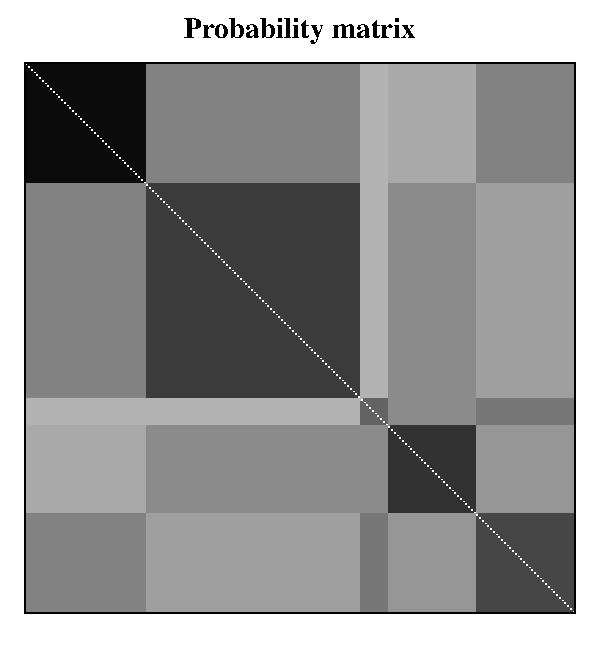
\includegraphics[width=\linewidth]{SBM_P.pdf}
\end{subfigure}%
\begin{subfigure}{.4\textwidth}
  \centering
  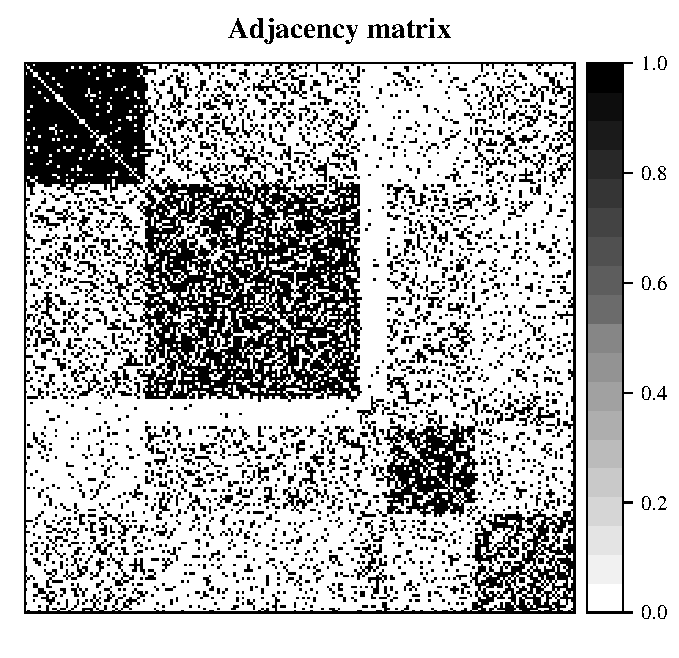
\includegraphics[width=\linewidth]{SBM_A.pdf}
\end{subfigure}
\begin{subfigure}{.4\textwidth}
  \centering
  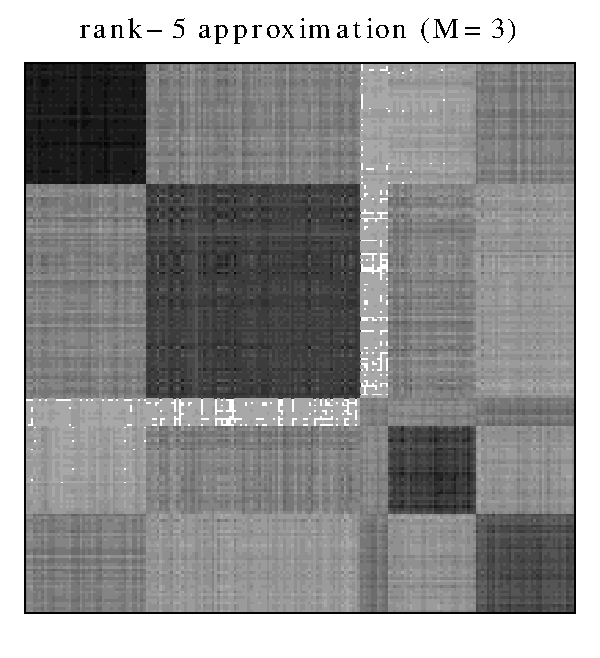
\includegraphics[width=\linewidth]{SBM_Phat.pdf}
\end{subfigure}%
\begin{subfigure}{.4\textwidth}
  \centering
  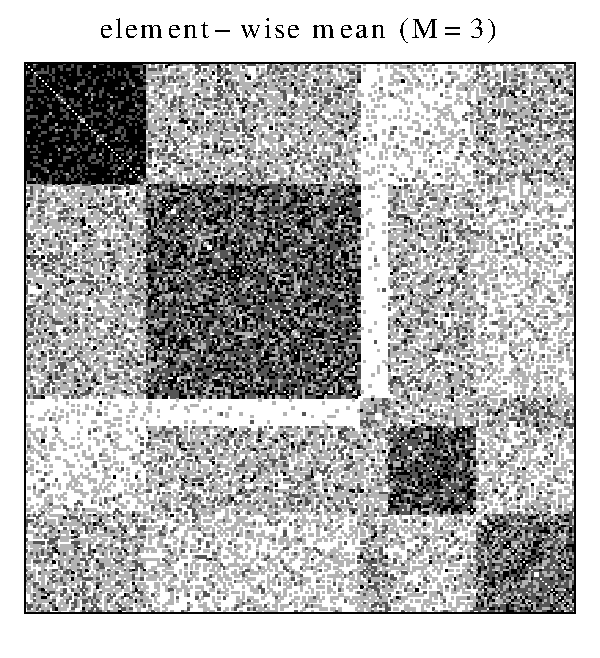
\includegraphics[width=\linewidth]{SBM_Abar.pdf}
\end{subfigure}
\caption{{\bf Example illustrating the stochastic blockmodel.}
The top left figure shows the mean graph $P$ with $K = 5$ blocks and $N=200$ vertices and the top right figure shows an adjacency matrix $A$ sampled according to the probabilities from $P$.
While $A$ is a noisy version of $P$, much of the structure of $P$ is preserved in $A$, a property we will exploit in our estimation procedure.
Based on three graphs sampled independently and identically according to the probability matrix $P$, we construct the element-wise mean $\bar{A}$, shown in the lower right panel (see Section~\ref{sec:abar}.  
Finally, by taking a rank-5 approximation of $\bar{A}$ and thresholding the values to be between $O$ and $1$, we construct our proposed estimate $\hat{P}$, shown in the lower left panel (see Section~\ref{sec:phat}).
By visual inspection, it is clear that the low-rank estimate $\hat{P}$ more closely approximates the probability matrix $P$ as compared to $\bar{A}$.
}
\label{fig:SBM_example}
\end{figure}


\subsection{Estimator $\bar{A}$}
\label{sec:abar}
The most natural estimator to consider is to take the average of the observed adjacency matrices which yields the element-wise sample mean.
This estimator, defined as $\bar{A}=\frac{1}{M}\sum_{m=1}^M A^{(m)}$, is the  maximum likelihood estimator (MLE) for the mean graph $P$ if the graphs are sampled from an IEM distribution.
It is unbiased so $\Ex[\bar{A}]=P$ with entry-wise variance $\mathrm{Var}(\bar{A}_{ij}) = P_{ij} (1-P_{ij})/M$. Moreover, $\bar{A}$ is the uniformly minimum-variance unbiased estimator, so it has the smallest variance among all unbiased estimators and enjoys the many asymptotic properties of the MLE as $M\to \infty$ for fixed $N$.
However, if graphs with a large number of vertices are of interest, there are no useful asymptotic properties for $\bar{A}$ as the number of vertices $N$ becomes large for fixed $M$.

Additionally, $\bar{A}$ doesn't exploit any graph structure.
If the graphs are distributed according to a RDPG or SBM, then $\bar{A}$ is no longer the maximum likelihood estimator since it is not guaranteed to satisfy the properties of the mean graph for that model.
The performance can be especially poor when the sample size $M$ is small, such as when $M\ll N$.
For example, when $M=1$, $\bar{A}$ is simple the binary adjacency matrix $A^{(1)}$, which is an inaccurate estimate for an arbitrary $P$ compared to estimates which exploit underlying structure, such as occurs for the RDPG.

\subsection{Low-Rank Estimator $\hat{P}$}
\label{sec:phat}

Motivated by the low-rank structure of the RDPG mean matrix, we propose the estimator $\hat{P}$ based on the spectral decomposition of $\bar{A}$ which yields a low rank approximation of $\bar{A}$.
This estimator is similar to the estimator proposed by \citet{chatterjee2015matrix} but additionally
we propose adjustments to canonical low-rank methods which serve to improve the performance for the specific task of estimating the mean graph. 
Additionally, we consider an alternative dimension selection technique as discussed in Section~\ref{section:dim_select}.

For a given dimension $d$ we consider the estimator $\mathrm{lowrank}(\bar{A})$ defined as the best rank-$d$ positive-semidefinite approximation of $\bar{A}$.
Since the graphs are symmetric, we can compute the eigen-decomposition of $\bar{A}$ as $\hat{U} \hat{S} \hat{U}^T + \tilde{U}\tilde{S}\tilde{U}^T$, where $\hat{S}$ is a diagonal matrix with non-increasing entries along the diagonal corresponding to the largest $d$ eigenvalues of $A$ and $\hat{U}$ has columns given by the corresponding eigenvectors.
The $d$-dimensional adjacency spectral embedding (ASE) of $\bar{A}$ is given by $\hat{X}=\hat{U} \hat{S}^{1/2}\in \Re^{N \times d}$.
For an RDPG, the rows of $\hat{X}$ are estimates of the latent vectors for each vertex \citep{sussman2014consistent}.
Using the adjacency spectral embedding, we have that the low-rank approximation of $\bar{A}$ is $\hat{X} \hat{X}^T=\hat{U}\hat{S}\hat{U}^T$.
Algorithm~\ref{algo:lowrank} gives the steps to compute this low-rank approximation.

\begin{algorithm}[H]
\caption{Algorithm to compute the rank-$d$ approximation of a matrix.}
\label{algo:lowrank}
\begin{algorithmic}[1]
\REQUIRE Symmetric matrix $A\in \Re^{N\times N}$ and dimension $d\leq N$.
\ENSURE $\mathrm{lowrank}_d(A)\in \Re^{N\times N}$
\STATE Compute the algebraically largest $d$ eigenvalues of $A$, $s_1>s_2>\dotsc,s_d$ and corresponding unit-norm eigenvectors $u_1,u_2,\dotsc,u_d\in \Re^N$;
\STATE Set $\hat{S}$ to the $d\times d$ diagonal matrix $\mathrm{diag}(s_1,\dotsc,s_d)$;
\STATE Set $\hat{U} = [u_1,\dotsc,u_d]\in \Re{N\times d}$;
\STATE Set $\mathrm{lowrank}_d(A)$ to $\hat{U}\hat{S}\hat{U}^T$;
\end{algorithmic}
\end{algorithm}

To compute our estimator $\hat{P}$, we need to additionally specify what rank $d$ to use and there are various ways of dealing with dimension selection. 
In this paper, we use Zhu and Ghodsi's elbow selection method \cite{zhu2006automatic} and the universal singular value thresholding (USVT) method \cite{chatterjee2015matrix}. 
Details for these methods are discussed in Section~\ref{section:dim_select}.

Moreover, since the adjacency matrices are hollow, with zeros along the diagonal, there is a missing data problem that leads to inaccuracies if we compute $\hat{P}$ based only on $\bar{A}$. 
To compensate for this issue, we use an iterative method developed by Scheinerman and Tucker \cite{scheinerman2010modeling}. 
Details are discussed in Section~\ref{section:diag_aug}.


\begin{algorithm}[H]
\caption{Algorithm to compute $\hat{P}$}
\label{algo:basic}
\begin{algorithmic}[1]
\REQUIRE Adjacency matrices $A^{(1)}, A^{(2)}, \cdots, A^{(M)}$, with each $A^{(m)} \in \{0,1\}^{N \times N}$
\ENSURE Estimate $\hat{P}\in[0,1]^{N\times N}$
\STATE Calculate the sample mean $\bar{A} = \frac{1}{M}\sum\limits_{m = 1}^M A^{(m)}$;
\STATE Calculate the scaled degree matrix $D^{(0)} = \mathrm{diag}(\bar{A} \bm{1})/(n-1)$;
\STATE Select the dimension $d$ based on the eigenvalues of $\bar{A} + D^{(0)}$; (see Section~\ref{section:dim_select})
\STATE Set $\tilde{P}^{(0)}$ to $\mathrm{lowrank}_d(\bar{A} + D^{(0)})$; (see Algorithm~\ref{algo:lowrank})
\STATE Set $D^{(1)}$ to $ \mathrm{diag}(\tilde{P})$, the diagonal matrix with diagonal matching $\tilde{P}$; 
\STATE Set $\tilde{P}^{(1)}$ to $\mathrm{lowrank}_d(\bar{A} + D^{(1)})$; (see Algorithm~\ref{algo:lowrank})
\STATE Set $\hat{P}$ to $\tilde{P}^{(1)}$ with values $<0$ set to $0$ and values $>1$ set to $1$.
\end{algorithmic}
\end{algorithm}


Algorithm~\ref{algo:basic} gives the steps involved to compute the low-rank estimate $\hat{P}$.
As we will see in the proceeding sections, this procedure will frequently yield improvements in estimation as compared to using the sample mean $\bar{A}$.
While this is unsurprising for random dot product graphs, where we are able to show theoretical results to this effect, we also see this effect for connectome data and more general independent edge graphs.
In the next sections, we explore this estimator in the context of the stochastic blockmodel.

The bottom panels of Fig.~\ref{fig:SBM_example} demonstrate the two estimators $\hat{P}$ and $\bar{A}$ for the stochastic blockmodel given by the upper left panel. 
The estimates are based on a sample of size $M=3$ and in this instance visual inspection demonstrates that $\hat{P}$ is performing significantly better than $\bar{A}$.



\section{Results}
\label{sec:result}

\subsection{Asymptotic Theory}
\label{section:theoretical_result}
To estimate the mean of a collection of graphs, we consider the two estimators from Section~\ref{section:model}: the entry-wise sample mean $\bar{A}$ and the low-rank $\hat{P}$ motivated by the RDPG.
In this section, we analyze the performance of these two estimators under the SBM by computing the entry-wise relative efficiency (RE), defined as $\mathrm{RE}(\bar{A}_{ij}, \hat{P}_{ij}) = \frac{\mathrm{MSE}(\hat{P}_{ij})}{\mathrm{MSE}(\bar{A}_{ij})}$.
Specifically, we consider the asymptotic relative efficiency as the number of vertices $N\to\infty$ but with the number of graphs $M$ fixed.
Somewhat surprising, the asymptotic relative efficiency will not depend on this fixed sample size $M$.

For this asymptotic framework, we assume where the block memberships $\tau_i$ are drawn iid from a multinomial distribution with block membership probabilities given by $\rho\in[0,1]^K$.
We will also assume that for a given $N$, the block membership probability are fixed for all graphs.
Denote block probability matrix $B = \nu \nu^T$. 
By definition, the mean of the collection of graphs generated from this SBM is $P$, where $P_{ij} = B_{\tau_i, \tau_j}$. After observing $M$ graphs on $N$ vertices $A^{(1)}, \cdots, A^{(M)}$ sampled independently from the SBM conditioned on $\tau$, we can calculate the two estimators $\bar{A}$ and $\hat{P}$.

\begin{lemma}
\label{lm:VarPhat}
For the above setting, for any $i, j$, if $\mathrm{rank}(B)=K=d$, we have
\[
    \lim_{N \to \infty} N \cdot \mathrm{Var}(\hat{P}_{ij}) =
    \frac{1/\rho_{\tau_i} + 1/\rho_{\tau_j}}{M} P_{ij} (1 - P_{ij}),
\]
and for large enough $N$, we have
\[
    \Ex[(\hat{P}_{ij} - P_{ij})^2] \approx
    \frac{1/\rho_{\tau_i} + 1/\rho_{\tau_j}}{M N} P_{ij}(1-P_{ij}).
\]
\end{lemma}
The first part of this Lemma gives the form the asymptotic variance of $\hat{P}$ and the second part ensures that additionally the estimator is approximately unbiased for $P$.
The proof of this lemma is outlined in Section~\ref{section:outline_proof} and is based on results for the variance of the adjacency spectral embedding from \citet{athreya2013limit}. From the result, we can see that the MSE of $\hat{P}_{ij}$ is of order $O(M^{-1}N^{-1})$ approximately.

Moreover, since $\bar{A}_{ij}$ is the sample mean of $M$ independent Bernoulli random variables with parameter $P_{ij}$, we have
\[
    \Ex[(\bar{A}_{ij} - P_{ij})^2] = \frac{P_{ij}(1-P_{ij})}{M}.
\]
This yields the following result.
\begin{theorem}
\label{thm:ARE}
In the same setting as in Lemma~\ref{lm:VarPhat}, for any $i$ and $j$, if $\mathrm{rank}(B)=K=d$, the asymptotic relative efficiency (ARE) is 
\[
    \mathrm{ARE}(\bar{A}_{ij}, \hat{P}_{ij}) = \lim_{N \to \infty} \mathrm{RE}(\bar{A}_{ij}, \hat{P}_{ij}) = 0.
    \label{eq:sbm_are}
\]
and for large enough $N$, we have
\begin{equation}
	    \mathrm{RE}(\bar{A}_{ij}, \hat{P}_{ij}) \approx
    \frac{1/\rho_{\tau_i} + 1/\rho_{\tau_j}}{N}.
\label{eq:approx_re}
\end{equation}
\end{theorem}


This theorem indicates that under the SBM, $\hat{P}$ is a much better estimate of the mean of the collection of graphs $P$ than $\bar{A}$.
Note, that a relative efficiency less than 1 indicates that $\hat{P}$ should be preferred over $\bar{A}$ so, under the above assumptions, as $N\to\infty$, $\hat{P}$ performs far better than $\bar{A}$.
From the result, we see that the relative efficiency is of order $O(N^{-1})$ and $N \cdot \mathrm{RE}(\bar{A}_{ij}, \hat{P}_{ij})$ converges to $1/\rho_{\tau_i}+1/\rho_{\tau_j}$ when $N$ goes to infinity.
An important aspect of Theorem~\ref{thm:ARE} is that the ARE does not depend on the number of graphs $M$, so the larger the graphs are, the better $\hat{P}$ is relative to $\bar{A}$, regardless of $M$.


The approximate formula Eq.~\ref{eq:approx_re} indicates that the the sizes of the blocks can greatly impact the relative efficiency.
To illustrate this consider a two block stochastic model. 
If each of the blocks contain half the vertices, then for each pair of vertices, the relative efficiency is approximately $4/N$. 
If the first block gets larger, with $\rho_1$ tending to 1, then the RE for estimating $P_{ij}$ with $\tau_i=\tau_j=1$, will tend to its minimum of $2/N$. 
On the other hand as $\rho_1\to 1$, if $\tau_i=1$ and $\tau_j=2$, then since $\rho_2=1-\rho_2$, the relative efficiency for estimating such an edge pair will be approximately $1$ and the same will hold if $\tau_i=\tau_j=2$.
Note that the maximum value for the relative efficiency in a two-block model is achieved when $\rho_1=1/N$ and $\rho_2=(N-1)/N$ in which case the relative efficiency is $(N^2+N-1)/N^2\approx 1$.
(Note values of $\rho_s$ below $1/N$ correspond to graphs where typically no vertices are in that block so the effective minimum we can consider for $\rho_s$ is $1/N$.)

% If for example there is one block containing half the vertices, the relative efficiency for estimating the probabilities of edges between vertices in that block will be approximately $4/N$.
% For even larger blocks, the relative efficiency will decrease towards $1/N$ as the proportion of the verties in that block tends.
% If a block has very few vertices, the asymptotic relative efficiency will tend towards one, but will always be less than one.
% x



\begin{figure}[!t]
\centering
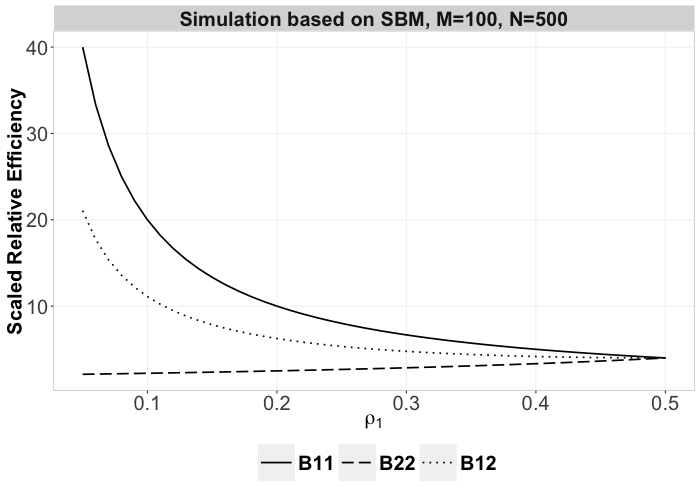
\includegraphics[width=1\textwidth]{Rho.pdf}
\caption{{\bf Asymptotic scaled relative efficiency $N\cdot RE(\bar{A},\hat{P})$ in a two-block SBM.}
For each distinct pair of edge probabilities in a two block model, the scaled relative efficiency only depends on the proportion of vertices in each block.
We show the scaled asymptotic relative efficiency as $\rho_1$ changes from $0,1$ for pairs of vertices where either both are in block 1 or one is in block one and one is in block two. 
These curves all intersect at a scaled relative efficiency of 4 when $\rho_1=1/2=\rho_2$.
Improvements using low-rank methods are greater for larger blocks, such as for $B_{11}$ when $\rho_1=$ is close to 1, while the improvements are smaller for block pairs with relatively few vertex pairs such as $B_{11}$ when $\rho_1$ is small and $B_{12}$ when $\rho_1$ is near 0 or 1
.
Note that the curve for $B_{22}$ would be the same as that for $B_{11}$ but reflected around the vertical line when $\rho_1=1/2$.
% Simulated results for scaled RE, i.e. $N \cdot \mathrm{RE}_{st}(\bar{A}, \hat{P})$ with $N = 500$ and $M = 100$ of 1000 Monte Carlo replicates while changing $\rho_1$ from 0.1 to 0.9. Scaled relative efficiency in average with different $N$ and fixed $M$ based on 1000 Monte Carlo replicates. Different types of lines denote the simulated values associated with the edges we are averaging over. Notice that when $\rho_1 = 0.5$, the scaled RE has value $4.0$, which agrees with the result in Fig~\ref{fig:RE} as expected.}
Overall, $\hat{P}$ performs best for large blocks while the improvements may be very minor for blocks with only a few vertices.
}
\label{fig:RErho}
\end{figure}



To illustrate Eq.~\ref{eq:approx_re} of Theorem~\ref{thm:ARE}, Fig.~\ref{fig:RErho} shows $2/\rho_1$ and $1/\rho_1+1/\rho_2$, the scaled asymptotic RE for pairs of vertices with block one and pairs of vertices in different blocks the blocks, respectively, in a  two-block stochastic blockmodel.
We vary $\rho_1$ between 0 and 1 to demonstrate how the number of pairs of vertices with the corresponding block memberships impacts the overall relative efficiency.
For $N=500$ and $M=100$, estimates of the scaled RE based on simulations agree very closely with their corresponding theoretical values displayed in the figure. Note that when $\rho_1 = 0.5$, the scaled RE has value $4.0$, which agrees with the result in Fig.~\ref{fig:RE} for simulated data.



If instead of assuming that the graphs follow a SBM distribution we assume the graphs are distributed according to a RDPG distribution, similar gains in relative efficiency can be realized.
While there is no compact analytical formula for the relative efficiency of $\hat{P}$ versus $\bar{A}$ in the general RDPG case, using the same ideas as in Theorem~\ref{thm:ARE}, we can show that $\mathrm{RE}(\bar{A}_{ij},\hat{P}_{ij}) = O(1/N)$.

\begin{proposition}
Suppose that $A^{(1)},A^{(2)},\dotsc,A^{(M)}$ are distributed iid from and RDPG distribution with common latent positions $X_1,\dotsc,X_n$, which are distributed iid from some distribution.
As the number of vertices $N$ tends to $\infty$, it holds for any $i\neq j$ that 
\[
    \mathrm{RE}(\bar{A}_{ij},\hat{P}_{ij}) \leq O(1/N).
\]
where again the asymptotic relative efficiency in $N$ does not depend on $M$.
\end{proposition}
The proof of this proposition closely follows the proofs of Lemma~\ref{lm:VarPhat} and Theorem~\ref{thm:ARE} and hence we omit it here.

\begin{remark}
As we noted above, if the graphs are distributed according to an SBM or an RDPG, the relative efficiency is approximately invariant to the number of graphs $M$ when $N$ is large.
If on the other hand, the graphs are generated according to a full-rank independent edge model, then the relative efficiency can change more dramatically as $M$ changes. 
The reason for this is because for larger $M$, more of the eigenvectors of $\bar{A}$ will begin to concentrate around the eigenvectors of the mean graph.
This leads to the fact that the optimal embedding dimension for estimating the mean will increase, making $\bar{A}$ and and the low-rank approximation at the optimal dimension closer together. 
As a result, $\mathrm{RE}(\bar{A},\hat{P})$ will increase as $M$ increases for full-rank models.
Indeed, for large $M$ we will have $\mathrm{RE}(\bar{A},\hat{P})$ since we cannot guarantee that $\hat{P}$ will choose the optimal dimension.
\end{remark}

\subsection{Finite Sample Simulations}\label{sec:sbm_sim}


\begin{figure}[!htb]
    \centering
    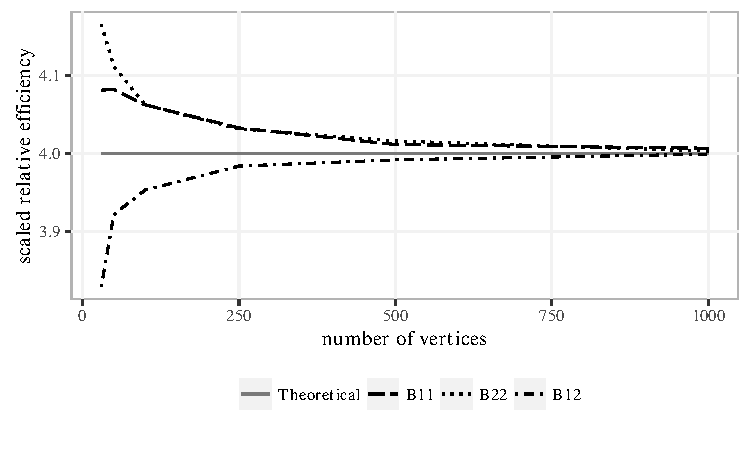
\includegraphics[width=1\textwidth]{RE.pdf}
    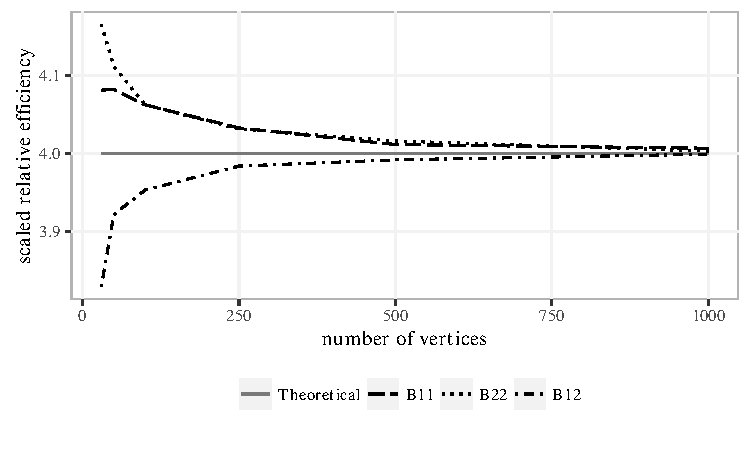
\includegraphics[width=1\textwidth]{scaled_RE.pdf}
    \caption{{\bf Finite sample relative efficiency based on simulations. }
    The top panel shows the estimated relative efficiency $\hat{\mathrm{RE}}(\bar{A},\hat{P})$ as a function of $N$ for fixed $M=100$ based on simulations of a SBM. 
    For each value of $N$, we used 1000 Monte Carlo replicates of the SBM from Section~\ref{sec:sbm_sim} to estimate the RE.
    Each curve corresponds to an average across vertex pairs corresponding the three distinct block probabilities, $B_{11}$, $B_{12}$, $B_{22}$ in the two-block SBM.
    Recall that values below 1 indicate that $\hat{P}$ is performing better than $\bar{A}$.
    The relative efficiencies are all very close so the lines are indistinguishable. \\
    To distinguish the three curves, the bottom panel shows the corresponding scaled relative efficiencies, $N\cdot \hat{RE}(\bar{A},\hat{P})$.
    The solid horizontal line indicates the theoretical asymptotic scaled relative which is  $1/\rho_s+1/\rho_t=4$, since $\rho_1=\rho_2=4$.
    All the curves converge quickly to this theoretical limit. }
    % Different types of dashed lines denote the simulated scaled RE associated with different blocks. Solid line represents the theoretical value for scaled RE. Observe that $N \cdot \mathrm{RE}_{st}(\bar{A}, \hat{P})$ converges to $1/\rho_s + 1/\rho_t = 4$ as expected.}
    \label{fig:RE}
\end{figure}

In this section, we will illustrate the theoretical results from Section 3.1 regarding the relative efficiency between $\bar{A}$ and $\hat{P}$ via Monte Carlo simulation experiments.
These numerical simulations will also allow us to investigate the finite sample performance of the two estimators.

%\subsubsection{Simulation Setting}
Here, we consider a 2-block SBM with parameters
\begin{equation*}
B = \begin{bmatrix}
0.42 & 0.2 \\
0.2 & 0.7
\end{bmatrix}
,\qquad \rho = \begin{bmatrix}
0.5 & 0.5
\end{bmatrix}.
\end{equation*}
When calculating $\hat{P}$, we omit the dimension selection step from Algorithm~\ref{algo:basic} and instead using the true dimension $d = \mathrm{rank}(B) = 2$.

%\subsubsection{Simulation Results}
To investigate the finite sample relative efficiency, we first sample 1000 Monte Carlo replicates from the above SBM distribution with different number of vertices $N$ and fixed number of graphs $M$. The  relative efficiency $\mathrm{RE}(\bar{A}_{ij}, \hat{P}_{ij})$ can be estimated since $P$ is known for this simulation. Since the relative efficiency only depends on the blocks memberships of the pair $i,j$, we estimate the relative efficiency for each block pair using
\[
    \hat{\mathrm{RE}}_{st}(\bar{A},\hat{P}) = \frac{\sum_{\tau_i=s,\tau_j=t,i \ne j} \hat{MSE}(\hat{P}_{ij})}{\sum_{\tau_i=s,\tau_j=t,i \ne j} \hat{MSE}(\bar{A}_{ij})}
\]
for $s,t\in\{1,2\}$, where $\hat{MSE}$ denotes the estimated mean square error based on the Monte Carlo replicates.
For the remaining simulations and real data analysis we will always be using estimated relative efficiency and estimated mean square error rather than analytic results and hence we will frequently omit that these are estimated values when it is clear from context.

In Fig.~\ref{fig:RE}, We plot the relative efficiency (top panel) and the scaled (estimated) relative efficiency (bottom panel), $N \cdot \hat{\mathrm{RE}}_{st}(\bar{A},\hat{P})$.
The different dashed lines denote the estimated scaled RE associated with different block pairs, either $B_{11}$, $B_{12}$ or $B_{22}$. 
As expected from Theorem~\ref{thm:ARE}, the top panel indicates that the relative efficiencies are all very close together and significantly less than 1, decreasing at the rate of $1/N$, indicating that $\hat{P}$ is performing better than $\bar{A}$.

Based on Theorem~\ref{thm:ARE}, we also have that the scaled RE converges to $1/\rho_{\tau_i}+1/\rho_{\tau_j}=4$ as $N\to\infty$ for all pairs $i,j$.
This is plotted as a solid line in the bottom panel.
From the figure, we see that $N \cdot \hat{\mathrm{RE}}_{st}(\bar{A}, \hat{P})$ converges to scaled asymptotic RE quite rapidly.
We omit error bars as the standard errors are very small for these estimates.
% {\color{red} Say something about why $B_{11}, B_{22}>4$ and $B_{12}<4$}

\begin{remark}
An intriguing aspect of these finite sample results is that the scaled relative efficiencies behave differently for small graphs with fewer vertices. 
The estimates of the edge probabilities for pairs of vertices in different blocks are significantly better than the estimates for edges within each block.
The reason for this is unclear and be due the actual values of the true probability, but it may also be do the fact there are approximately twice as many pairs of vertices in different blocks $N^2/4$, than there are in the same block, $N^2/8-N/4$.
This could lead to an increase in effective sample size which may cause the larger differences displayed in the left parts of Fig.~\ref{fig:RE}.
However, overall these differences are nearly indistinguishable for unscaled relative efficiency.
\end{remark}


\subsection{CoRR Brain Graphs: Cross-Validation}\label{sec:corr_data}

In practice, graphs do not follow the independent edge model, let alone an RDPG or SBM, but the mean of a collection of graphs is still of interest for these cases.
To demonstrate that the estimator $\hat{P}$ is still useful in such cases, we test its performance on structural connectomic data. 
The graphs are based on diffusion tensor MR images collected and available at the Consortium for Reliability and Reproducibility (CoRR) \citep{zuo2014open, gorgolewski2015high} (see Section~\ref{section:data}).

The dataset contains 454 different brain scans, each of which was processed to yield an undirected, unweighted graph with no self-loops, using the pipeline describe in \citet{gray2013migraine} and \citet{kiar2016m2g}.
The vertices of the graphs represent different regions in the brain defined according to an atlas.
We used three atlases, the JHU atlas with 48 vertices, the Desikan atlas with 70 vertices and the  CPAC200 atlas with 200.
An edge exists between two vertices whenever there is at least one white-matter tract connecting the corresponding two regions of the brain. 
Further details of the dataset are provided in Section~\ref{section:data}.

In order to evaluate the performance of the two estimators, we use a cross validation on the 454 graphs of each size. 
Specifically, for a given atlas, each Monte Carlo replicate corresponds to sampling $M$ graphs out of the 454 and computing the low-rank estimator $\hat{P}$ and the sample mean $\bar{A}$ using the $M$ selected graphs. 
We then compare these estimates to the sample mean for the remaining $454-M$ adjacency matrices.
While we cannot interpret this mean graph as the probability matrix for an IEM distribution (see Section~\ref{sec:sim_iem}), the sample mean for the remaining graphs does give the proportion of times each pair of vertices are adjacent in the population from which the graphs were sampled.

While in previous sections we evaluated the mean square error for either an individual entry or for an entire block in the SBM, in this section and the next section we will focus on the overall error for estimating the mean graph.
In particular we will use the average of the mean square error across all pairs of vertices and we define $MSE(\bar{A}) = \binom{N}{2}^{-1} \sum_{i>j}\Ex[\bar{A}_{ij}-P_{ij}]$ and similarly for $\mathrm{MSE}(\hat{P})$.
As in the previous section, we will not use analytical evaluations of the MSE and instead estimate the MSE and relative efficiencies via Monte Carlo simulations.
% By observing 454 graphs generated by the atlas being picked, we use $\hat{P}$ to estimate the mean graph $P$, which is the proportions of the existence of a white-matter tract connecting different parts of the brain. Since $P$ is unknown in practice, we perform a cross-validation study to compare $\bar{A}$ and $\hat{P}$. For each Monte Carlo replicate, we first fix the sample size $M$ and randomly sample $M$ graphs from the total 454 graphs in the dataset. We assure $M$ to be relatively small such that the entry-wise mean of the remaining $(454 - M)$ graphs is a valid approximation of the true probability matrix $P$ we are estimating. Then we can calculate $\bar{A}$ and $\hat{P}$ based on the $M$ samples and compare their performance based on the estimated probability matrix.

We run 1000 simulations on each of the three atlases for each sample size $M=1,5,10$.
We also considered all possible dimensions for $\hat{P}$ by ranging $d$ from 1 to $N$ in order to investigate the impact of the dimension selection procedures.
We plot $\hat{MSE}$ of $\bar{A}$ and $\hat{P}$ in Fig.~\ref{fig:realdata}.
The horizontal axis gives dimension $d$, which only impacts $\hat{P}$, which is why estimated MSE of $\bar{A}$ is shown as flat.

When $d$ is small, $\hat{P}$ underestimate the dimension and throws away important information, which leads to relatively poor performance. When $d=N$, $\hat{P}$ is equal to $\bar{A}$, so that the curve for $\hat{MSE}$ for $\hat{P}$ ends at $\hat{MSE}(\bar{A})$. 
In practice, we use algorithms like Zhu and Ghodsi's method or USVT to select the dimension $d$ (see Section~\ref{section:dim_select}). 
In the figure, we denote the 3rd elbow found by the Zhu and Ghodsi method by a triangle , and denote the dimension selected by USVT with threshold 0.7 by a square. 
% (with largest 95\% confidence interval length to be $3.5$)
% (with largest 95\% confidence interval length to be $0.7$) 
Both dimension selection algorithms tend to select dimensions which nearly minimize the mean square error.
% The standard error for the Zhu and Ghodsi and the USVT methods are about $0.9$ and $0.17$ respectively.

When $M$ is 1 or 5, $\bar{A}$ has large variance which leads to large $\hat{\mathrm{MSE}}$. Meanwhile, $\hat{P}$ reduces the variance by taking advantages of inherent low-rank structure of the mean graph. Additionally, we see that there is a large range of dimensions where the performance for $\hat{P}$ is superior to $\bar{A}$. 
With a larger $M$, the performance of $\bar{A}$ improves so that its performance is frequently superior but nearly identical to $\hat{P}$.

For a more specific comparison of the performance of $\hat{P}$ and $\bar{A}$ in the most realistic situation where the rank $d$ much be chosen based on data, Table~\ref{tab:corr_re} shows estimated relative efficiencies of $\hat{P}$ versus $\bar{A}$.
For each atlas and each sample size we compare the \citet{zhu2006automatic} with the USVT method and note that both perform reasonable well relative to the full-dimensional $\bar{A}$.
We omit confidence intervals for the estimated relative efficiencies since all confidence intervals had lengths less than $0.015$, indicating that all relative efficiencies are significantly different from 1.

Again we can see that the largest improvements using $\hat{P}$ occur when $m$ is small and $N$ is large. 
On the other hand, once $m=10$, $\bar{A}$ tends to do nearly as well or better than $\hat{P}$. 
Nonetheless, $\hat{P}$ offers certain advantages, especially since low-rank estimates can often be more easily interpretable by considering the latent position representation described in Section~\ref{section:sbm_rdpg}.

\begin{figure}[!htb]
\centering
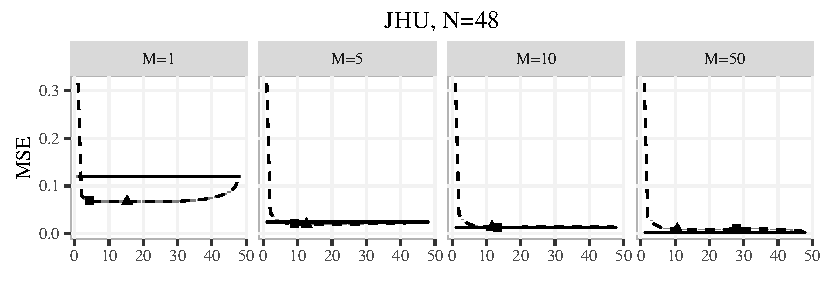
\includegraphics[width=1\textwidth]{corr_data_MSE_jhu.pdf}\\
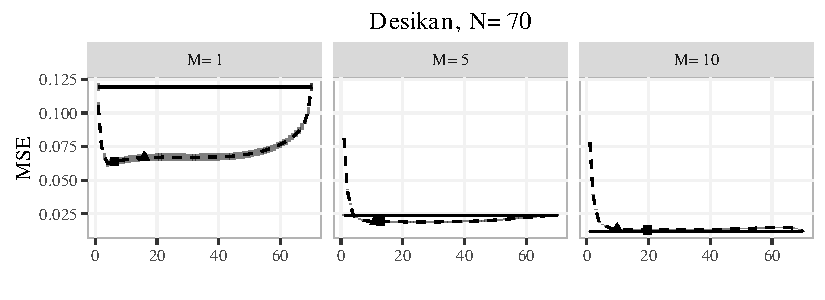
\includegraphics[width=1\textwidth]{corr_data_MSE_desikan.pdf}\\
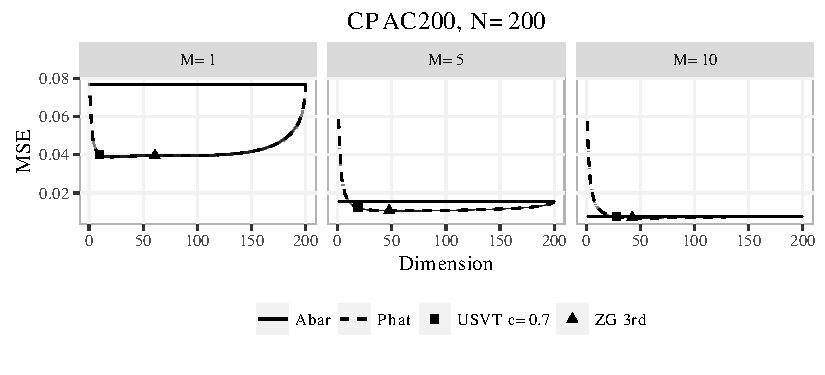
\includegraphics[width=1\textwidth]{corr_data_MSE_CPAC200.pdf}
\caption{{\bf Comparison of $\hat{\mathrm{MSE}}$ of $\hat{P}$ and $\bar{A}$ for three atlases at three sample sizes for the CoRR data.}
These plots show the mean square error for $\bar{A}$ (solid line) and $\hat{P}$ (dashed line) for three dataset (JHU, Desikan and CPAC200) while embedding the graphs into different dimensions and with different sample sizes $M$. The average dimensions chosen by the 3rd elbow of Zhu and Ghodsi is denoted by a triangle
 % (with largest 95\% confidence interval length to be $3.5$), 
 and chosen by USVT with threshold equals 0.7 is denoted in square.
% (with largest 95\% confidence interval length to be $0.7$). 
 Vertical intervals, visible mainly in the $N=48,70$ and $M=1$ plots, represent the 95\% confidence interval for the mean square errors.  When $M$ is small, $\hat{P}$ outperforms $\bar{A}$ with a flexible range of the embedding dimension including the average of the dimensions selected by Zhu and Ghodsi and USVT.}
\label{fig:realdata}
\end{figure}

\begin{table}[!htb]
    \caption{{\bf Relative efficiencies of $\bar{A}$ versus $\hat{P}$ for the CoRR data set.}
    For each atlas, JHU, Desikan, and CPAC 200, we sampled graphs which we used to compute $\bar{A}$ and $\hat{P}$.
     We compared different sample sizes $m$ and different dimension selection procedures, ZG and USVT.
    For each of the two methods for computing $\hat{P}$, we estimated their relative efficiencies with respect to the sample mean $\bar{A}$.
    Confidence intervals all had lengths less than $0.015$ and hence we omitted them for clarity.
    Overall, the relative efficiencies are greater for smaller sample sizes $m$ and larger number of vertices $N$. 
    } 
    \label{tab:corr_re}
    \centering

\begin{tabular}{rccc}\toprule
        % & $m=1$  & $m=5$  & $m=10$ \\\toprule
\multicolumn{1}{l}{\textbf{JHU}} & $m=1$  & $m=5$  & $m=10$  \\\midrule
ZG      & 0.54 & 0.81 & 1.14 \\
USVT    & 0.56 & 0.84 & 1.12 \\\midrule
\multicolumn{1}{l}{\textbf{Desikan}} & $m=1$  & $m=5$  & $m=10$  \\ \midrule
ZG      & 0.52 & 0.81 & 1.14 \\
USVT    & 0.50 & 0.81 & 1.09 \\\midrule
\multicolumn{1}{l}{\textbf{CPAC200}} & $m=1$  & $m=5$  & $m=10$  \\\midrule
ZG      & 0.51 & 0.68 & 0.89 \\
USVT    & 0.52 & 0.79 & 0.99 \\\bottomrule
\end{tabular}
\end{table}



To further illustrate the differences between the two estimators, we consider a single random sample of size $M=5$ based on the Desikan atlas.
We calculated $\bar{A}$ and $\hat{P}$, using  Zhu and Ghodsi's 3rd elbow to select $d=11$. 
In Fig.~\ref{fig:Matrix_desikan_m5}, the estimates $\bar{A}$ and $\hat{P}$ as well as the sample mean of 454 graphs (as a close estimate of $P$) are plotted. 
Since the sample size is small, there are a lot of pairs of vertices with no edges or 5 edges in the 5 observations.
This leads to the white and black pixels in the image corresponding to $\bar{A}$.
On the other hand, $\hat{P}$ has a finer gradient of values which in this case leads to a more accurate estimate.

Moreover, Fig.~\ref{fig:Diff_desikan_m5} shows the values for the absolute estimation error $|\bar{A} - P|$ and $|\hat{P}-P|$. The lower triangular sections shows the actual absolute difference while the upper triangular matrix highlights the vertex pairs with absolute differences larger than 0.4. 
There are 18 edges from $\bar{A}$ and 6 edges from $\hat{P}$ being highlighted in the figure, further indicating the superior performance of $\hat{P}$.
Note that $\approx 13\%$ of the potential edges are present in all $454$ graphs and hence $\bar{A}$ will always have zero error for those pairs of vertices.
Nonetheless, $\hat{P}$ typically outperforms $\bar{A}$.

To investigate the difference in performance with respect to the geometry of brain, 
in Fig.~\ref{fig:Diff_between_desikan}, we plot the 50 edges with the largest difference $|\bar{A} - P| - |\hat{P} - P|$ according to the location of the corresponding regions in the brain. Red edges indicate that $\hat{P}$ overestimate $P$ while blue means that $\hat{P}$ underestimate $P$. The edge width is determined by the estimation error for $\hat{P}$, where pairs with larger estimation error are represented by thicker lines.
We also highlight the five regions corresponding to vertices that contribute most to the difference, meaning the vertices $i$ with the largest value of $\sum_j (|\bar{A} - P| - |\hat{P} - P|)_{ij}$.
Notably, these regions of improvement appear to be concentrated in three distinct regions of the brain. 
The top five regions are the inferior temporal, middle temporal, and transverse temporal regions in the left hemisphere and the parahippocampal and parsopercularis regions in the right hemisphere of the Desikan atlas.

These results demonstrate that for small sample sizes, such as $M=1$ or $M=5$, and for the atlases with larger number of vertices, $\hat{P}$ gives a better estimate than $\bar{A}$ for the CoRR dataset.
Importantly, this improvement is robust to the embedding dimension provided the dimension is not underestimated.
We should note that though the total error for $\hat{P}$ is smaller in this case, for certain entries $\bar{A}$ does perform better.
For example, there are some pairs of vertices that are adjacent for all samples in the population and for these pairs $\bar{A}$ will always perform better than $\hat{P}$. 

\begin{figure}[!htb]
\centering
\includegraphics[height=.18\textheight]{P_desikan.pdf} 
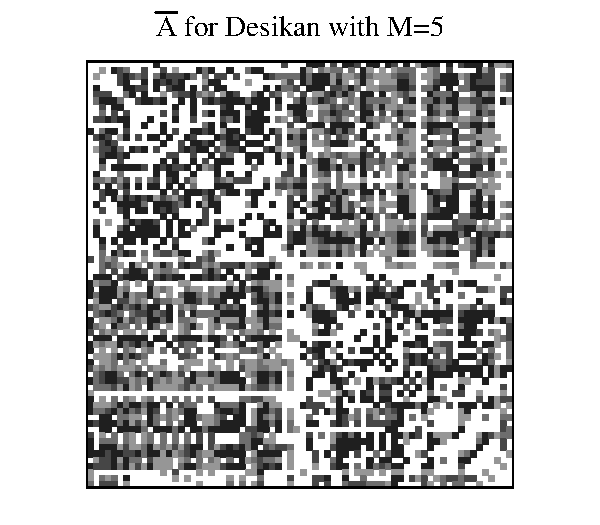
\includegraphics[height=.182\textheight]{Abar_desikan_m5.pdf} 
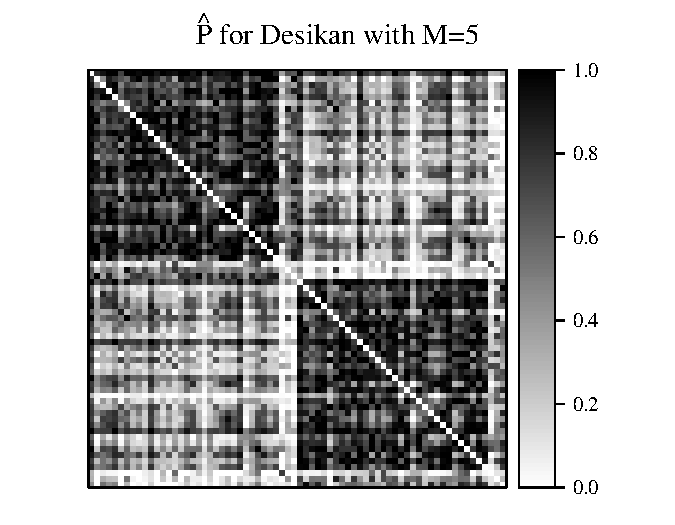
\includegraphics[height=.186\textheight]{Phat_desikan_m5.pdf}
\caption{{\bf Heat maps of the population mean, the sample mean, the the estimator $\hat{P}$.}
These heat maps indicate the sample mean for the remaining $454-5$ graphs (left), sample mean for the 5 sampled graphs (center), and $\hat{P}$ for the 5 sampled graphs with dimension $d=11$ selected using the Zhu and Ghodsi method (right).
Darker pixels indicated a higher probability of an edge between the given vertices.
Note that $\hat{P}$ appears to be better estimate the true probabilities $P$, especially for edges between the two hemispheres, in the upper right (and lower left) block.
}
\label{fig:Matrix_desikan_m5}
\end{figure}

\begin{figure}

\begin{center}
  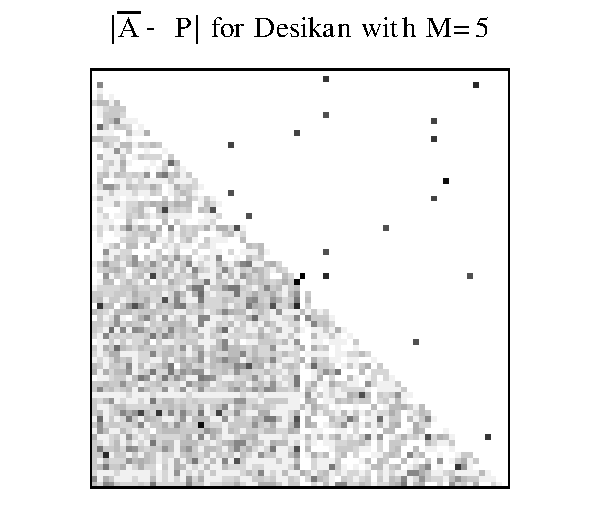
\includegraphics[height=.4\linewidth]{Diff2_desikan_m5.pdf}\hspace{-12pt}
  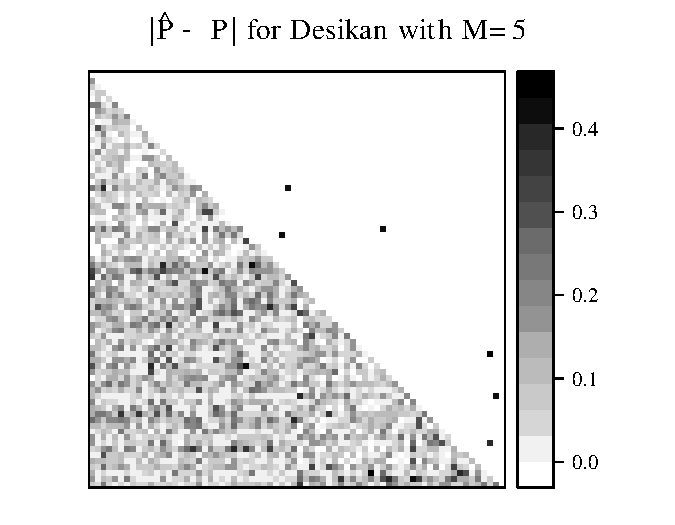
\includegraphics[height=.4\linewidth]{Diff3_desikan_m5.pdf}
\end{center}

\caption{{\bf Heat plot of absolute estimation error for $\bar{A}$ and $\hat{P}$ (lower triangle) and absolute errors above 0.4 (upper triangle).}
These heat plots show the absolute estimation error $|\bar{A} - P|$ and $|\hat{P} - P|$ for a sample of size $M=5$ from Desikan dataset.
The embedding dimension for $\hat{P}$ is $d=11$ selected by the 3rd elbow for ZG method. The lower triangular matrix shows the actual absolute difference, while the upper triangular matrix only highlights the edges with absolute differences larger than $0.4$. The fact that 18 edges from $\bar{A}$ are highlighted and while only six edges from $\hat{P}$ are highlighted indicates that $\hat{P}$ suffers from fewer large outliers.}
\label{fig:Diff_desikan_m5}
\end{figure}

\begin{figure}[!htb]
\centering
\includegraphics[width=1\textwidth]{Diff_between_desikan.png}
\caption{{\bf Top 5 regions of the brain (vertices in graphs) and top 50 connections between regions (edges in graphs) with largest difference $|\bar{A} - P| - |\hat{P} - P|$.}
Red edges indicate that $\hat{P}$ overestimate $P$ while blue means that $\hat{P}$ underestimate $P$. The edge width is determined by the estimation error. Connections with larger estimation error are represented by thicker lines. This figure shows the regions and connections of the brain where $\hat{P}$ outperforms $\bar{A}$ the most for estimating $P$.}
\label{fig:Diff_between_desikan}
\end{figure}


%\begin{figure}[!htb]
%\centering
%\includegraphics[width=1\textwidth]{JHU.png}
%\caption{Comparison of MSE between $\bar{A}$ (solid line) and $\hat{P}$ (dashed line) for JHU dataset while embedding the graphs into different dimensions with different size $M$ of the subsamples. The dimension chosen by the 3rd elbow of Zhu and Ghodsi is denoted in triangle, and chosen by USVT with threshold equals 0.7 is denoted in square. Vertical intervals represent the 95\% confidence interval. When $M$ is small, $\hat{P}$ outperforms $\bar{A}$ with a flexible range of the embedding dimension including what Zhu and Ghodsi selects.}
%\label{fig:JHU}
%\end{figure}
%
%\begin{figure}[!htb]
%\centering
%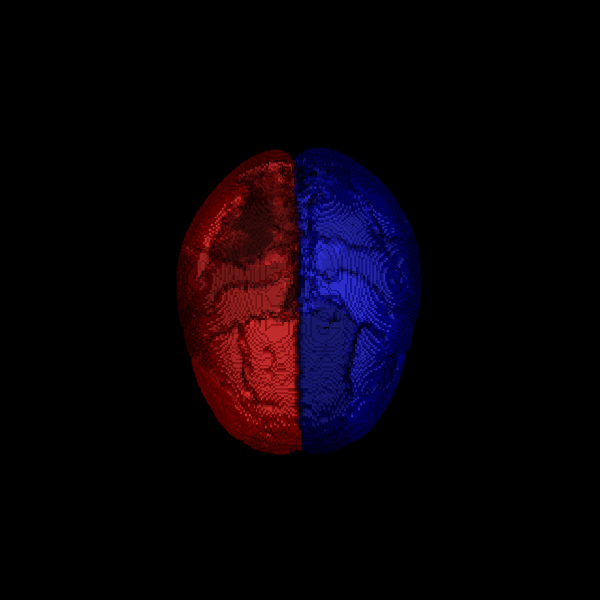
\includegraphics[width=1\textwidth]{desikan.png}
%\caption{Comparison of MSE between $\bar{A}$ (solid line) and $\hat{P}$ (dashed line) for desikan dataset while embedding the graphs into different dimensions with different size $M$ of the subsamples. The dimension chosen by the 3rd elbow of Zhu and Ghodsi is denoted in triangle, and chosen by USVT with threshold equals 0.7 is denoted in square.  Vertical intervals represent the 95\% confidence interval.  When $M$ is small, $\hat{P}$ outperforms $\bar{A}$ with a flexible range of the embedding dimension including what Zhu and Ghodsi selects.}
%\label{fig:desikan}
%\end{figure}
%
%\begin{figure}[!htb]
%\centering
%\includegraphics[width=1\textwidth]{CPAC200.png}
%\caption{Comparison of MSE between $\bar{A}$ (solid line) and $\hat{P}$ (dashed line) for CPAC200 dataset while embedding the graphs into different dimensions with different size $M$ of the subsamples. The dimension chosen by the 3rd elbow of Zhu and Ghodsi is denoted in triangle, and chosen by USVT with threshold equals 0.7 is denoted in square.  Vertical intervals represent the 95\% confidence interval.  When $M$ is small, $\hat{P}$ outperforms $\bar{A}$ with a flexible range of the embedding dimension including what Zhu and Ghodsi selects.}
%\label{fig:CPAC200}
%\end{figure}
%
%\begin{figure}
%\centering
%\begin{subfigure}{.33\textwidth}
%  \centering
%  \includegraphics[width=1.2\linewidth]{P_JHU.png}
%\end{subfigure}%
%\begin{subfigure}{.33\textwidth}
%  \centering
%  \includegraphics[width=1.2\linewidth]{Abar_JHU_m5.png}
%\end{subfigure}
%\begin{subfigure}{.33\textwidth}
%  \centering
%  \includegraphics[width=1.2\linewidth]{Phat_JHU_m5.png}
%\end{subfigure}
%\caption{Comparison between the mean of 454 graphs $P$ and two estimates $\bar{A}$ and $\hat{P}$ derived from a sample of size $M=5$ from JHU dataset while embedding the graphs into dimension $d=15$ selected by the 3rd elbow of ZG method.}
%\label{fig:adj_JHU_m5}
%\end{figure}
%
%\begin{figure}[!htb]
%\centering
%\includegraphics[width=1\textwidth]{Vertex_Diff_Phat_desikan.png}
%\caption{Top 5 regions of the brain (vertices in graphs) with largest absolute difference $|\hat{P} - P|$.}
%\label{fig:Vertex_Diff_Phat_desikan}
%\end{figure}
%
%\begin{figure}[!htb]
%\centering
%\includegraphics[width=1\textwidth]{Edge_Diff_Phat_desikan.png}
%\caption{Top 1\% (49) connections between regions (edges in graphs) with largest absolute difference $|\hat{P} - P|$.}
%\label{fig:Vertex_Diff_Phat_desikan}
%\end{figure}


\subsection{Synthetic Data Analysis for Full Rank IEM}\label{sec:sim_iem}

While the theory we have developed is based on the assumption that the mean graph is low rank, as we have seen in Section~\ref{sec:corr_data}, $\hat{P}$ often performs well even when this assumption is false. 
To further illuminate this point, we perform a synthetic data analysis under a full-rank independent edge model where we use the sample mean of the 454 graphs in the Desikan dataset as the probability matrix $P$.
As in the previous section, we simulated data sets of size $M=1,5$, and $10$ and used $\bar{A}$ and $\hat{P}$, where for $\hat{P}$ we varied the rank from 1 to 70.

Fig.~\ref{fig:sim_desikan} shows resulting estimated MSE for $\bar{A}$ (solid line) and $\hat{P}$ (dashed line) for simulated data based on the full rank probability matrix $P$ shown in the left panel of Fig.~\ref{fig:Matrix_desikan_m5}.
% Vertical lines at each dimension indicate the 95\% confidence intervals for the MSE.
We see that the results are very similar to those presented in Section~\ref{sec:corr_data}, though overall $\hat{P}$ performs even better than in the real data experiments. 
When $M$ is small, $\hat{P}$ outperforms $\bar{A}$ with a flexible range of the embedding dimension including those selected by the Zhu and Ghodsi method while when $M$ is large enough, both estimators perform well with the decision between the two being less conclusive.
This simulation again shows the robustness of $\hat{P}$ to deviations from the RDPG model, specifically if the probability matrix is full-rank.

We also note that the finite-sample relative efficiency in these cases shows is even more favorable to $\hat{P}$, with relative efficiencies lower than $1/3$ for $M=1$, than for the real data, where relative efficiencies were at best around $1/2$ for $M=1$.
From this observation we can postulate that the degradation in the performance of $\hat{P}$ in real data can at least partially be attributed to the fact that the independent edge assumption does not hold for real data.


\begin{figure}[!htb]
\centering
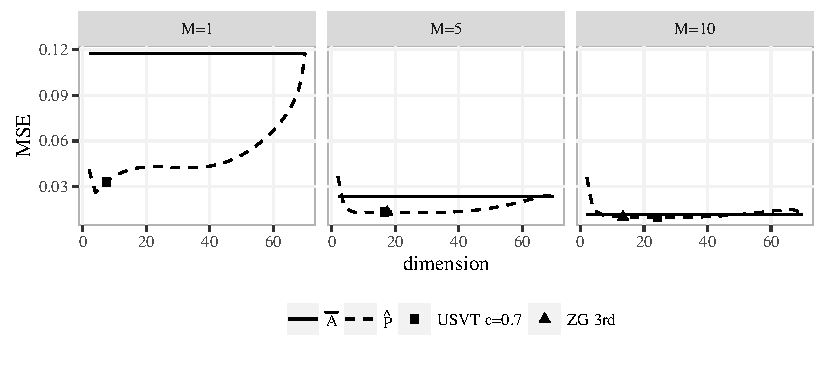
\includegraphics[width=1\textwidth]{sim_desikan.pdf}
\caption{{\bf Comparison of $\hat{P}$ and $\bar{A}$ for synthetic data analysis.}
As in Fig.~\ref{fig:RE}, this figure show $\hat{\mathrm{MSE}}$ for $\bar{A}$ (solid line) and $\hat{P}$ (dashed line) for simulated data with different sample sizes $M$ based on the sample mean for the Desikan dataset. Again, the average of dimensions selected by the USVT method (square) and the ZG method (triangle) tend to nearly approximate the optimal dimension. 
Overall, we see that the structure of these plots well approximates the structure for the real data indicating that performance for the independent edge model will tend to translate in structure to non-independent edge scenarios. 
On the other hand, the relative efficiency $\hat{\mathrm{RE}}(\bar{A},\hat{P})$ is lower for this synthetic data analysis then for the CoRR data.}
\label{fig:sim_desikan}
\end{figure}



\section{Discussion}\label{sec:discussion}

% In this paper, we propose using low-rank methods to estimate the mean of a collection of graphs.
Motivated by the RDPG model, our methodology takes advantage of the low-rank structure of the graphs by applying low-rank approximation to the entry-wise MLE. 
We give a closed form for the asymptotic relative efficiency between the entry-wise MLE $\bar{A}$ and our estimator $\hat{P}$ in the case of a stochastic blockmodel, demonstrating that when the number of vertices $N$ is sufficiently large, low-rank methods provide a substantial improvement.
In particular, we show that for a stochastic blockmodel with fixed number of blocks $K$, block size proportion $\rho$, and number of graphs $M$, the low-rank estimator $\hat{P}$ has MSE which is on the order of $N$ times lower than the MSE for $\bar{A}$.

Moreover, our estimator outperforms the entry-wise MLE in a cross validation analysis of the CoRR brain graphs and in low- and full-rank simulation settings.
These results illustrate that $\hat{P}$ performs well even when the low-rank assumption is violated and that $\hat{P}$ is robust and can be applied in practice.

One of the key observations from our real data analysis was that the largest improvements using the low-rank method occurred when the number of graphs $M$ was small and that it provided only minor improvements or degrade performance slightly when $M$ is large. 
However, even in large scale studies the low-rank methods will be useful for estimating graph means for subpopulations, for example the population of females over 60 with some college education.
Using the element-wise sample mean for such small strata, which may have fewer than ten subjects, will frequently result in a degradation of performance.
In similar direction, \citet{durante2014nonparametric} used low-rank deviations from a full rank population mean to model collections of graphs and our methods could be easily adapted to these ideas.

We also note that low-rank methods can often be more easily interpreted.
By representing a low-rank matrix in terms of the latent position, where each vertex is represented as a vectors in $\Re^d$ and the entries of the matrix are given by inner products of these vectors (see Section~\ref{section:sbm_rdpg}), one can analyze and visualize the geometry of these vectors in order to interpret how each vertex is behaving in the context of the larger graph. 
Additionally, such a representation allows the use of techniques from multivariate analysis to further study the estimated population mean.



% \subsection{Future Work}
% In this paper, we assume that the adjacency matrix is observed without contamination.
% However, generally there will be noise in practice and accounting for this noise with other more robust methods . With contaminations, robust estimators like ML$q$E is preferred. If an estimator can not only inherit robustness from the robust estimators but also has small variance by taking advantage of the low rank structure of the graphs, it will be very useful.

% Meanwhile, estimating the rank of the graph structure accurately will certainly help improve the performance of the estimator $\hat{P}$. Now we are using Zhu and Ghodsi's method and USVT, but there is still a lot of space for improvement, especially in this particular case.

While the low-rank methods considered in this paper will often offer substantial improvements, further refinements of these methods which account for the particular traits of connectomics data would be useful to improve estimation further.
For example, we assume that the adjacency matrix is observed without contamination, however, in practice there will be noise in the observed graph and one may seek to account for this noise with more robust methods.
This may be especially fruitful when each graph has weighted edges and the weights themselves have noisy or heavy-tailed distributions.
Rank-based methods and robust likelihood methods could be very useful in that case \citep{huber2009robust,qin2013maximum}. 

 % With contaminations, robust estimators like ML$q$E is preferred. If an estimator can not only inherit robustness from the robust estimators but also has small variance by taking advantage of the low rank structure of the graphs, it will be very useful.

Another issue that arose in our analysis of the connectome data set was the presence of structural ones in the mean graph for the population. 
These structural ones appear since edges between certain regions of the brain are present in all or nearly all members of the healthy population. 
The low-rank methods tend to miss these always present edges while the sample mean will always capture them.
Detecting and incorporating structural ones and zeros could yield methods that share the best elements of both methods considered here.

For the CoRR data set, we used a cross validation framework where we compared the estimates based on a subsample to the mean for the held-out set. 
Another option would be to compare the estimates $\bar{A}$ and $\hat{P}$ to the mean for the entire population including the subsample.
Both of these analyses lead to very similar results in the cases presented above but for various reasons one may prefer one analysis over another.
The cross validation method is most reasonable from a prediction perspective where prediction about new samples is of interest.
If instead, one is interested in learning directly about the mean of a population, especially a finite population, the sub-sampling approach may be the most logical choice.

\section{Methods}
\label{sec:method}

\subsection{Choosing Dimension}
\label{section:dim_select}
Often in dimensionality reduction techniques, the choice for dimension $d$, relies on analyzing the set of the ordered eigenvalues, looking for a ``gap'' or ``elbow'' in the scree-plot. \citet{zhu2006automatic} present an automated method for finding this gap in the scree-plot that takes only the ordered eigenvalues as an input and uses Gaussian mixture modeling to find these gaps.
The mixture modeling results in multiple candidate dimensions or elbows and our analysis indicated that underestimating the dimension is much more harmful than overestimating the dimension.
For this reason, we use the 3rd elbow in the experiments performed in this work.

Universal Singular Value Thresholding (USVT) is a simple estimation procedure proposed by \citet{chatterjee2015matrix} that can work for any matrix that has ``a little bit of structure''. 
In our setting, it selects the dimension $d$ as the number singular values that are greater than a constant $c$ times $\sqrt{N/M}$.
The specific constant $c$ must be selected carefully based on the mean and variance of the entries and since again we found that overestimating the dimension was not overly harmful, we chose a relatively small value of $c=0.7$.

Overall, selecting the appropriate dimension is a challenging task and numerous methods could be applied successfully depending on the setting.
On the other hand, we have observed that in our setting many dimensions will yield nearly optimal mean square errors and so efforts to ensure the selected dimension are in the appropriate range are more important than finding the singular best dimension.



\subsection{Graph Diagonal Augmentation}
\label{section:diag_aug}
The graphs examined in this work have no self-loops and thus the diagonal entries of the adjacency matrix and the mean graph are all zero.
However, when computing the low-rank approximation, these structural zeros lead to increased errors in the estimation of the mean graph. 
While this problem has been investigated in the single graph setting, with multiple graphs, the problem is exasperated since the variance of the others entries is lower, so the relative impact of the bias in the diagonal entries is higher.

\citet{marchette2011vertex}  proposed the simple method of imputing the diagonals to be equal to the average of the non-diagonal entries for the corresponding row.
Earlier, \citet{scheinerman2010modeling} proposed using an iterative method to impute the diagonal entries.
In this work we combine these two ideas by first using the row-average method  (see Step 3 of Algorithm~\ref{algo:basic}) and then using one step of the iterative method (see Step 6 of Algorithm~\ref{algo:basic}).
Note that when computing errors, we omit the diagonal entries since these are known to be zero.

\subsection{Mean Square Error and Relative Efficiency}
\label{section:rel_eff}
We evaluate our estimators in terms of mean square error, either $\mathrm{MSE}(\hat{P}_{ij})=\Ex[\hat{P}_{ij}-P]^2$ or $\mathrm{MSE}(\bar{A})=\Ex[\bar{A}_{ij}-P]^2$.
While we can directly compare the difference in mean square errors between the two estimators, it is frequently useful to consider the relative efficiency between two estimators.
In our case this is $\mathrm{RE}(\bar{A}_{ij},\hat{P}_{ij}) = \frac{\mathrm{MSE}(\hat{P}_{ij})}{\mathrm{MSE}(\bar{A}_{ij})}$, with values above 1 indicating $\bar{A}$ should be preferred while values below 1 indicate $\hat{P}$ should be preferred.
We also use asymptotic relative efficiency, which is the limit of the relative efficiency as the number of vertices increase to infinity, and the scaled relative efficiency, $N\cdot \mathrm{RE}(\bar{A}_{ij},\hat{P}_{ij}) $ which in our case normalizes the relative efficiency so that the asymptotic scaled relative efficiency is non-zero and finite.
Relative efficiency is a useful metric for comparing estimators because it will frequently be invariant to the scale of the noise in the problem and hence is more easily comparable across different settings.

\subsection{Dataset Description}
\label{section:data}
The original dataset is from the Emotion and Creativity One Year Retest Dataset provided by Qiu, Zhang and Wei from Southwest University available at the Consortium for Reliability and Reproducibility (CoRR) \cite{zuo2014open, gorgolewski2015high}. It is comprised of 235 subjects, all of whom were college students. Each subject underwent two sessions of anatomical, resting state DTI scans, spaced one year apart. Due to incomplete data, only 454 are available.

When deriving MR connectomes, the NeuroData team parcellates the brain into groups of voxels as defined by anatomical atlases \cite{neurodata, kiar2016graph}. The atlases are defined either physiologically by neuroanatomists (Desikan and JHU), or are generated using an automated segmentation algorithm (CPAC200).
% The graphs we are using are processed by NeuroData team from DTI data of the original dataset generated with different atlases (Desikan, JHU and CPAC200), each containing different region/node definitions. 
Once the voxels in the original image space are grouped into regions, an edge is placed between two regions when there is at least one white-matter tract, derived using a tractography algorithm, connecting the corresponding two parts of the brain.
The resulting graphs are undirected, unweighted and have no self-loops.


\subsection{Outline for the Proof of the Theorems}
\label{section:outline_proof}
Here we provide an outline of the proof Lemma~\ref{lm:VarPhat} which provides the approximate MSE of $\hat{P}$ in the stochastic blockmodel case.
The result depends on using the asymptotic results for the distribution of eigenvectors from \citet{athreya2013limit} which extend to the multiple graph setting in a straightforward way.

The first key observation, is that since $\bar{A}$ is computed from iid observations each with expectation $P$, $\bar{A}$ is unbiased for $P$ and $\mathrm{Var}(A_{ij}) = \frac{1}{M}P_{ij}(1-P_{ij}$.
The results of \citet{athreya2013limit} provide a central limit theorem for estimates of the latent position in a RDPG model for a single graph.
Since the variance of each entry is scaled by $1/M$ in $\bar{A}$, the analogous result for $\bar{A}$ is that the estimated latent positions will follow an approximately normal distribution with variance scaled by $1/M$ compared to the variance for a single graph. 
    
% When comparing two estimators, the first thing we need to consider is consistency.
% It is easy to see that $\bar{A}$ is unbiased as an estimate of $P$. 
% Moreover, since two latent positions are conditionally asymptotically independent by extended version of Theorem 1 in \citet{athreya2013limit}, we know $\hat{P}$ is consistent, as well as $\bar{A}$.

% Thus the relative efficiency between $\hat{P}$ and $\bar{A}$, which is equivalent to the ratio of mean square errors in this case, is a good indicate in comparison.

Since $\hat{P}_{ij} = \hat{X}_i^T \hat{X}_j$ is a noisy version of the dot product of $\nu_s^T \nu_t$ from Section~\ref{section:sbm_rdpg} and each $\hat{X}_i$ are approximately independent and normal, we can use common results for the variance of the inner product of two independent multivariate normals \citep{brown1977means}.
After simplifications that occur in the stochastic blockmodel setting we can derive that the variance of $\hat{P}_{ij}$ converges to $\left( 1/\rho_{\tau_i} + 1/\rho_{\tau_j} \right) P_{ij} (1-P_{ij})/(N \cdot M)$ as $N \rightarrow \infty$. 
Since the variance of $\bar{A}_{ij}$ is $P_{ij} (1-P_{ij})/M$, the relative efficiency between $\hat{P}_{ij}$ and $\bar{A}_{ij}$ is approximately $(\rho_{\tau_i}^{-1} + \rho_{\tau_j}^{-1})/N$ when $N$ is sufficiently large.
    

\section*{Acknowledgments}

This work is graciously supported by the XDATA program of the Defense
Advanced Research Projects Agency (DARPA) administered through Air
Force Research Laboratory contract FA8750-12-2-0303; the DARPA SIMPLEX
program through SPAWAR contract N66001-15-C-4041; and DARPA GRAPHS
contract N66001-14-1-4028.

\nolinenumbers

% Either type in your references using
% \begin{thebibliography}{}
% \bibitem{}
% Text
% \end{thebibliography}
%
% or
%
% Compile your BiBTeX database using our plos2015.bst
% style file and paste the contents of your .bbl file
% here.
% 
\begin{thebibliography}{10}
\providecommand{\natexlab}[1]{#1}
\providecommand{\url}[1]{\texttt{#1}}
\expandafter\ifx\csname urlstyle\endcsname\relax
  \providecommand{\doi}[1]{doi: #1}\else
  \providecommand{\doi}{doi: \begingroup \urlstyle{rm}\Url}\fi

\bibitem[neu()]{neurodata}
Neurodata’s mri to graphs pipeline.
\newblock \url{http://m2g.io}.
\newblock Accessed: 2016-05-23.

\bibitem[Athreya et~al.(2013)Athreya, Priebe, Tang, Lyzinski, Marchette, and
  Sussman]{athreya2013limit}
Avanti Athreya, CE~Priebe, M~Tang, V~Lyzinski, DJ~Marchette, and DL~Sussman.
\newblock A limit theorem for scaled eigenvectors of random dot product graphs.
\newblock \emph{Sankhya A}, pages 1--18, 2013.

\bibitem[Bollob{\'a}s et~al.(2007)Bollob{\'a}s, Janson, and
  Riordan]{bollobas2007phase}
B{\'e}la Bollob{\'a}s, Svante Janson, and Oliver Riordan.
\newblock The phase transition in inhomogeneous random graphs.
\newblock \emph{Random Structures \& Algorithms}, 31\penalty0 (1):\penalty0
  3--122, 2007.

\bibitem[Brown and Rutemiller(1977)]{brown1977means}
Gerald~G Brown and Herbert~C Rutemiller.
\newblock Means and variances of stochastic vector products with applications
  to random linear models.
\newblock \emph{Management Science}, 24\penalty0 (2):\penalty0 210--216, 1977.

\bibitem[Chatterjee et~al.(2015)]{chatterjee2015matrix}
Sourav Chatterjee et~al.
\newblock Matrix estimation by universal singular value thresholding.
\newblock \emph{The Annals of Statistics}, 43\penalty0 (1):\penalty0 177--214,
  2015.

\bibitem[Durante et~al.(2014)Durante, Dunson, and
  Vogelstein]{durante2014nonparametric}
Daniele Durante, David~B Dunson, and Joshua~T Vogelstein.
\newblock Nonparametric bayes modeling of populations of networks.
\newblock \emph{arXiv preprint arXiv:1406.7851}, 2014.

\bibitem[Ginestet et~al.(2014)Ginestet, Balanchandran, Rosenberg, and
  Kolaczyk]{ginestet2014hypothesis}
Cedric~E Ginestet, Prakash Balanchandran, Steven Rosenberg, and Eric~D
  Kolaczyk.
\newblock Hypothesis testing for network data in functional neuroimaging.
\newblock \emph{arXiv preprint arXiv:1407.5525}, 2014.

\bibitem[Gorgolewski et~al.(2015)Gorgolewski, Mendes, Wilfling, Wladimirow,
  Gauthier, Bonnen, Ruby, Trampel, Bazin, Cozatl, et~al.]{gorgolewski2015high}
Krzysztof~J Gorgolewski, Natacha Mendes, Domenica Wilfling, Elisabeth
  Wladimirow, Claudine~J Gauthier, Tyler Bonnen, Florence~JM Ruby, Robert
  Trampel, Pierre-Louis Bazin, Roberto Cozatl, et~al.
\newblock A high resolution 7-tesla resting-state fmri test-retest dataset with
  cognitive and physiological measures.
\newblock \emph{Scientific data}, 2, 2015.

\bibitem[Gutmann(1982)]{gutmann1982stein}
Sam Gutmann.
\newblock Stein's paradox is impossible in problems with finite sample space.
\newblock \emph{The Annals of Statistics}, pages 1017--1020, 1982.

\bibitem[Hoff et~al.(2002)Hoff, Raftery, and Handcock]{hoff2002latent}
Peter~D Hoff, Adrian~E Raftery, and Mark~S Handcock.
\newblock Latent space approaches to social network analysis.
\newblock \emph{Journal of the american Statistical association}, 97\penalty0
  (460):\penalty0 1090--1098, 2002.

\bibitem[Holland et~al.(1983)Holland, Laskey, and
  Leinhardt]{holland1983stochastic}
Paul~W Holland, Kathryn~Blackmond Laskey, and Samuel Leinhardt.
\newblock Stochastic blockmodels: First steps.
\newblock \emph{Social networks}, 5\penalty0 (2):\penalty0 109--137, 1983.

\bibitem[Huber and Ronchetti(2009)]{huber2009robust}
Peter~J. Huber and Elvezio~M. Ronchetti.
\newblock \emph{Robust statistics}.
\newblock Wiley Series in Probability and Statistics. John Wiley \& Sons, Inc.,
  Hoboken, NJ, second edition, 2009.

\bibitem[James and Stein(1961)]{james1961estimation}
W.~James and Charles Stein.
\newblock Estimation with quadratic loss.
\newblock In \emph{Proceedings of the {F}ourth {B}erkeley {S}ymposium on
  {M}athematical {S}tatistics and {P}robability, {V}ol. {I}}, pages 361--379.
  Univ. California Press, Berkeley, Calif., 1961.

\bibitem[Jiang et~al.(2001)Jiang, M{\"u}unger, and Bunke]{jiang2001median}
Xiaoyi Jiang, Andreas M{\"u}unger, and Horst Bunke.
\newblock On median graphs: Properties, algorithms, and applications.
\newblock \emph{IEEE Transactions on Pattern Analysis and Machine
  Intelligence}, 23\penalty0 (10):\penalty0 1144--1151, 2001.

\bibitem[Kiar(2016)]{kiar2016graph}
Gregory Kiar.
\newblock Gremlin: Graph estimation from mr images leading to inference in
  neuroscience.
\newblock 2016.

\bibitem[Kiar et~al.(In Preparation)Kiar, Roncal, Mhembere, Bridgeford, Burns,
  Priebe, and Vogelstein]{kiar2016m2g}
Gregory Kiar, William~Gray Roncal, Disa Mhembere, Eric Bridgeford, Randal
  Burns, Carey Priebe, and Joshua~T. Vogelstein.
\newblock m2g: A reliable and robust open-source one-click pipeline for mri to
  graph connectome estimation.
\newblock In Preparation.

\bibitem[Marchette et~al.(2011)Marchette, Priebe, and
  Coppersmith]{marchette2011vertex}
David Marchette, Carey Priebe, and Glen Coppersmith.
\newblock Vertex nomination via attributed random dot product graphs.
\newblock In \emph{Proceedings of the 57th ISI World Statistics Congress},
  volume~6, page~16, 2011.

\bibitem[Nickel(2007)]{nickel2007random}
Christine Leigh~Myers Nickel.
\newblock \emph{Random dot product graphs: A model for social networks},
  volume~68.
\newblock 2007.


\bibitem[Qin and Priebe(2013)]{qin2013maximum}
Yichen Qin and Carey~E Priebe.
\newblock Maximum l q-likelihood estimation via the expectation-maximization
  algorithm: A robust estimation of mixture models.
\newblock \emph{Journal of the American Statistical Association}, 108\penalty0
  (503):\penalty0 914--928, 2013.

\bibitem[Roncal et~al.(2013)Roncal, Koterba, Mhembere, Kleissas, Vogelstein,
  Burns, Bowles, Donavos, Ryman, Jung, Wu, Calhoun, and
  Vogelstein]{gray2013migraine}
W.~Gray Roncal, Z.~H. Koterba, D.~Mhembere, D.~M. Kleissas, J.~T. Vogelstein,
  R.~Burns, A.~R. Bowles, D.~K. Donavos, S.~Ryman, R.~E. Jung, L.~Wu,
  V.~Calhoun, and R.~J. Vogelstein.
\newblock Migraine: Mri graph reliability analysis and inference for
  connectomics.
\newblock In \emph{Global Conference on Signal and Information Processing
  (GlobalSIP), 2013 IEEE}, pages 313--316, Dec 2013.
\newblock \doi{10.1109/GlobalSIP.2013.6736878}.

\bibitem[Scheinerman and Tucker(2010)]{scheinerman2010modeling}
Edward~R Scheinerman and Kimberly Tucker.
\newblock Modeling graphs using dot product representations.
\newblock \emph{Computational Statistics}, 25\penalty0 (1):\penalty0 1--16,
  2010.

\bibitem[Stein(1956)]{stein1956inadmissibility}
Charles Stein.
\newblock Inadmissibility of the usual estimator for the mean of a multivariate
  normal distribution.
\newblock In \emph{Proceedings of the {T}hird {B}erkeley {S}ymposium on
  {M}athematical {S}tatistics and {P}robability, vol. {I}}, pages 197--206.
  University of California Press, Berkeley and Los Angeles, 1956.

\bibitem[Sussman et~al.(2014)Sussman, Tang, and Priebe]{sussman2014consistent}
Daniel~L Sussman, Minh Tang, and Carey~E Priebe.
\newblock Consistent latent position estimation and vertex classification for
  random dot product graphs.
\newblock \emph{IEEE transactions on pattern analysis and machine
  intelligence}, 36\penalty0 (1):\penalty0 48--57, 2014.

\bibitem[Trunk(1979)]{trunk1979problem}
G.~V. Trunk.
\newblock A problem of dimensionality: A simple example.
\newblock \emph{Pattern Analysis and Machine Intelligence, IEEE Transactions
  on}, \penalty0 (3):\penalty0 306--307, 1979.


\bibitem[Young and Scheinerman(2007)]{young2007random}
Stephen~J Young and Edward~R Scheinerman.
\newblock Random dot product graph models for social networks.
\newblock In \emph{Algorithms and models for the web-graph}, pages 138--149.
  Springer, 2007.

\bibitem[Zhu and Ghodsi(2006)]{zhu2006automatic}
Mu~Zhu and Ali Ghodsi.
\newblock Automatic dimensionality selection from the scree plot via the use of
  profile likelihood.
\newblock \emph{Computational Statistics \& Data Analysis}, 51\penalty0
  (2):\penalty0 918--930, 2006.

\bibitem[Zuo et~al.(2014)Zuo, Anderson, Bellec, Birn, Biswal, Blautzik,
  Breitner, Buckner, Calhoun, Castellanos, et~al.]{zuo2014open}
Xi-Nian Zuo, Jeffrey~S Anderson, Pierre Bellec, Rasmus~M Birn, Bharat~B Biswal,
  Janusch Blautzik, John~CS Breitner, Randy~L Buckner, Vince~D Calhoun,
  F~Xavier Castellanos, et~al.
\newblock An open science resource for establishing reliability and
  reproducibility in functional connectomics.
\newblock \emph{Scientific data}, 1, 2014.

\end{thebibliography}

\appendix

\section{Proofs for Theory Results}
Here we present the proofs of the results in from Section~\ref{section:theoretical_result}. To keep the ideas clear and concise, we leave out some details which are only slight changes to previous works.
We assume the block memberships $\tau_i$ are drawn iid from a multinomial distribution with block membership probabilities given by $\rho\in[0,1]^K$ where $\sum_i \rho_=1$.
We will also assume that for a given $N$, the block memberships are fixed for all graphs.

Denote matrix of between block edge probabilities by $B = \nu \nu^T\in[0,1]^{K\times K}$ which we assume has rank $k$ and is positive definite. 
By definition, the mean of the collection of graphs generated from this SBM is $P$, where $P_{ij} = B_{\tau_i, \tau_j}$. 

We observe $M$ graphs on $N$ vertices $A^{(1)}, \cdots, A^{(M)}$ sampled independently from the SBM conditioned on $\tau$.
Define $\bar{A} = \frac{1}{m} \sum_{t=1}^m A^{(t)}$. Let $\hat{U} \hat{S} \hat{U}^T$ be the best rank-$d$ positive semidefinite approximation of $\bar{A}$, then we define $\hat{P} = \hat{X} \hat{X}^T$, where $\hat{X} = \hat{U} \hat{S}^{1/2}$.




The proofs presented here will rely on a central limit theorem developed in \citet{athreya2013limit}. 
We modify the Theorem slightly to account for the multiple graph setting and present it in the special case of the stochastic blockmodel.

\begin{theorem}[Corrolary of Theorem 1 in \citet{athreya2013limit}]\label{thm:clt_ext}
  In the setting above, let $X=[X_1,\dotsc,X_N]^T\in\Re^{K\times d}$ have row $i$ equal to $X_i=\nu_{\tau_i}$ where recall that $\tau_i$ are drawn from $[K]$ according to the probabilities $\rho$.
	Then there exists an  orthogonal matrices $W$ such that for each row $i$ and $j$ and any $z \in \Re^{d}$, conditioned on $\tau_i=s$ and $\tau_j=t$,
  \begin{equation}
    \label{eq:4}
    \Pr\left\{\sqrt{n}( W \hat{X}_i - \nu_s ) \leq z, \sqrt{n}( W \hat{X}_j - \nu_t) \leq z'\right\}
=  \Phi(z, \Sigma(\nu_s)/M)  \Phi(z', \Sigma(\nu_t)/M) +o(1)
  \end{equation}
  where $\Sigma(x) =\Delta^{-1}\Ex[ X_j X_j^\top(x^\top X_j -(x^\top
  X_j)^2)]\Delta^{-1}$ and $\Delta=\Ex[ X_1 X_{1}^{T}]$ is the second
  moment matrix, with all expectations taken unconditionally.
  The function $\Phi$ is the cumulative distribution function for a multivariate normal with mean zero and the specified covariance and $o(1)$ denotes a function that tends to zero as $N\to \infty$.
\end{theorem}
The proof of this result follows very closely the proof of the result in the original paper with only slight modifications for the multiple graph setting.

We now prove a technical Lemma which yields the simplified form for the variance under the stochastic blockmodel.

\begin{lemma}
\label{lm:mseForm}
In the same setting as Theorem~\ref{thm:ARE}, for any $1 \le s, t \le K$, we have
\[
	\nu_s^T \Sigma(\nu_t) \nu_s = \frac{1}{\rho_s} \nu_s^T \nu_t (1- \nu_s^T \nu_t).
\]
\end{lemma}
\begin{proof}
Under the stochastic block model with parameters $(B, \rho)$, we have $X_i \stackrel{iid}{\sim} \sum_{k=1}^K \rho_k \delta_{\nu_k}$, where $\nu = [\nu_1, \cdots, \nu_K]^T$ satisfies $B = \nu \nu^T$. Without loss of generality, we could assume that $\nu = U S$ where $U = [u_1, \cdots, u_K]^T$ is orthonormal in columns and $S$ is a diagonal matrix. Here we can conclude that $\nu_s^T = u_s^T S$. Also define $R = \text{diag}(\rho_1, \cdots, \rho_K)$, then we have
\[
	\Delta = E[X_1 X_1^T] = \sum_{k=1}^K \rho_k \nu_k \nu_k^T = \nu^T R \nu = S U^T R U S.
\]
Thus
\begin{align*}
	\nu_s^T \Sigma(\nu_t) \nu_s = &
    \nu_s^T \Delta^{-1} \sum_{k=1}^K \rho_k \nu_k \nu_k^T (\nu_t^T \nu_k)(1 - \nu_t^T \nu_k) \Delta^{-1} \nu_s \\
    = & \sum_{k=1}^K \rho_k (\nu_s^T \Delta^{-1} \nu_k) (\nu_k^T \Delta^{-1} \nu_s) (\nu_t^T \nu_k) (1 - \nu_t^T \nu_k) \\
    = & \sum_{k=1}^K \rho_k (u_s^T U^T R^{-1} U u_k)^2 (\nu_t^T \nu_k) (1 - \nu_t^T \nu_k) \\
    = & \sum_{k=1}^K \rho_k (e_s^T R^{-1} e_k)^2 (\nu_t^T \nu_k) (1 - \nu_t^T \nu_k) \\
    = & \sum_{k=1}^K \rho_k \delta_{sk} \rho_s^{-2} (\nu_t^T \nu_k) (1 - \nu_t^T \nu_k) \\
    = & \frac{1}{\rho_s} \nu_t^T \nu_s (1 - \nu_t^T \nu_s)
\end{align*}
\end{proof}

% \subsection{Parameter Setting}
% Under SBM($B, \rho$) with $n$ vertices and $K$ blocks, we have the $d$-dimensional latent position $X_i \stackrel{iid}{\sim} \sum_{k=1}^K \rho_k \delta_{\nu_k}$, where $d = \mathrm{rank}(B) \le K$ and $\nu = [\nu_1, \cdots, \nu_K]^T \in \Re^{K \times d}$ satisfying $B = \nu \nu^T$. Define the block assignment $\tau$ such that $\tau_i = k$ if and only if $X_i = \nu_k$. Let $P = X X^T$ where $X = [X_1, \cdots, X_n]^T$.
% Here we assume that the second moment matrix for $X_i$, $\Delta = E[X_i X_i^T]$, is diagonal without loss of generality. Moreover, we assume that the eigenvalues of $\Delta$ are distinct and positive for the remainder of this work.

% First draw $\tau \in [K]^n$ from the multinomial distribution with parameter $\rho$. Then we sample $m$ conditionally i.i.d.~graphs $A^{(1)}, \cdots, A^{(m)}$ such that $A^{(t)}_{ij}|\tau \stackrel{ind}{\sim} Bern(P_{ij})$ for each $1 \le t \le m$, $1 \le i, j \le n$.



% \subsection{Asymptotic Relative Efficiency}

% When two reasonable estimators $S$ and $T$ of the parameter $\theta$ are considered, we always want to know which one is preferred. When both of them are unbiased, the one with a smaller variance would be more efficient. So if $\{S_n\}$ and $\{T_n\}$ are asymptotic unbiased for $\theta$, then define the asymptotic relative efficiency of $\{S_n\}$ with respect to $\{T_n\}$ to be
% \[
% 	\mathrm{ARE}(S_n, T_n) = \lim_{n \rightarrow \infty} \frac{Var(T_n)}{Var(S_n)}.
% \]
% An extended version of ARE is that, when $\{S_n\}$ and $\{T_n\}$ are sequences of estimators for $\theta$ (not necessarily to be asymptotic unbiased), then define the asymptotic relative efficiency of $\{S_n\}$ with respect to $\{T_n\}$ to be
% \[
% 	\mathrm{ARE}(S_n, T_n) = \lim_{n \rightarrow \infty} \frac{Var(T_n)/E[T_n]^2}{Var(S_n)/E[S_n]^2}.
% \]


\begin{lemma}[Lemma~\ref{lm:VarPhat}]
In the same setting as above, for any $i, j$, conditioning on $X_i = \nu_{\tau_i}$ and $X_j = \nu_{\tau_j}$, we have
\[
	\lim_{N \to \infty} N \cdot \mathrm{Var}(\hat{P}_{ij}) =
    \frac{1/\rho_{\tau_i} + 1/\rho_{\tau_j}}{M} P_{ij} (1 - P_{ij}).
\]
And for $N$ large enough, conditioning on $X_i = \nu_{\tau_i}$ and $X_j = \nu_{\tau_j}$, we have
\[
	E[(\hat{P}_{ij} - P_{ij})^2] \approx
    \frac{1/\rho_{\tau_i} + 1/\rho_{\tau_j}}{M N} P_{ij}(1-P_{ij}).
\]
\end{lemma}
\begin{proof}
% In Athreya et al. (2013), Theorem 4.8 states that conditioned on $X_i = \nu_k$, there
% exists a sequence of orthogonal matrices $W_n$ converging to the identity almost surely such that
% $P \left( \sqrt{n} (W_n \hat{X}_i - \nu_k) \le z | X_i = \nu_k \right) \rightarrow \Phi(z, \Sigma(x_i))$ as $n \rightarrow \infty$, where $\Sigma(x) = \Delta^{-1} E[X_j X_j^T (x^T X_j)(1 - x^T X_j)] \Delta^{-1}$, $\Delta = E[X_1 X_1^T]$ and $\Phi(z, \Sigma)$ denotes the cumulative distribution function for the multivariate normal, with mean zero and covariance matrix $\Sigma$, evaluated at $z$. Thus the sequence of random variables $\sqrt{n}(W_n \hat{X}_i - \nu_k)$ converges in distribution to a normal distribution.
Conditioned on $X_i = \nu_k$, we have by Theorem~\ref{thm:clt_ext},
\[
	E[W \hat{X}_i] = \nu_k+o(1)
\]
and
\[
	n \cdot \mathrm{Cov}(W \hat{X}_i, W_n \hat{X}_i) = \Sigma(\nu_k)/M.
\]

% The results above are actually based on the \href{https://www.overleaf.com/2962543bbfkxq}{extended version of Avanti's CLT}.

Also, Corollary 4.11 in Athreya et al. (2013) says $\hat{X}_i$ and $\hat{X}_j$ are asymptotically independent. Thus conditioning on $X_i = \nu_s$ and $X_j = \nu_t$, we have $\lim_{n\to\infty}E[\hat{X}_i^T \hat{X}_j] = \lim_{n\to\infty}E[(W_n \hat{X}_i)^T] E[W_n \hat{X}_j] = \nu_s^T \nu_t = P_{ij}$.

Since $\hat{P}_{ij} = \hat{X}_i^T \hat{X}_j$ is a noisy version of the dot product of $\nu_s^T \nu_t$, combined with Lemma~\ref{lm:mseForm} and the results above, by Equation 5 in Brown and Rutemiller (1977), conditioning on $X_i = \nu_s$ and $X_j = \nu_t$, we have
\[
	E[\hat{X}_i^T \hat{X}_j] = E[(W_n \hat{X}_i)^T] E[W_n \hat{X}_j] = \nu_s^T \nu_t+o(1) = P_{ij}+o(1)
\]
and
\begin{align*}
	& n \cdot \mathrm{Var} (\hat{P}_{ij}) \\
    = & \frac{1}{m} \left( \nu_s^T \Sigma(\nu_t) \nu_s + \nu_t^T \Sigma(\nu_s) \nu_t^T \right)
    + \frac{1}{m^2 n} \left( tr(\Sigma(\nu_s) \Sigma(\nu_t)) \right) +o(1)\\
    = & \frac{1}{m} \left( \nu_s^T \Sigma(\nu_t) \nu_s + \nu_t^T \Sigma(\nu_s) \nu_t^T \right)+o(1) \\
    = & \frac{1/\rho_s + 1/\rho_t}{m} P_{ij}(1-P_{ij}) + o(1).
\end{align*}
Since $\hat{P}_{ij} = \hat{X}_i^T \hat{X}_j$ is asymptotically unbiased for $P_{ij}$, when $n$ is large enough, we have
\[
    E[(\hat{P}_{ij} - P_{ij})^2] = \mathrm{Var}(\hat{P}_{ij}) \approx
    \frac{1/\rho_s + 1/\rho_t}{m n} P_{ij}(1-P_{ij})+o(1).
\]
\end{proof}





% \begin{theorem}
% \label{thm:ARE}
% For any $i$ and $j$, conditioning on $X_i = \nu_{\tau_i}$ and $X_j = \nu_{\tau_j}$, we have
% \[
% 	\mathrm{ARE}(\bar{A}_{ij}, \hat{P}_{ij}) = 0.
% \]
% And for $n$ large enough, conditioning on $X_i = \nu_{\tau_i}$ and $X_j = \nu_{\tau_j}$, we have
% \[
% 	\mathrm{RE}(\bar{A}_{ij}, \hat{P}_{ij}) \approx
%     \frac{1/\rho_{\tau_i} + 1/\rho_{\tau_j}}{n}.
% \]
% \end{theorem}
% \begin{proof}
% Since $A^{(t)}_{ij}$ ($1 \le t \le m$) are i.i.d. Bernoulli random variables with parameter $P_{ij}$, we have
% \[
% 	\mathrm{Var}(\bar{A}_{ij}) = \frac{1}{m} P_{ij} (1 - P_{ij}).
% \]
% Combined with Lemma \ref{lm:VarPhat}, we have
% \[
% 	\mathrm{ARE}(\bar{A}_{ij}, \hat{P}_{ij})
%     = \lim_{n \to \infty} \frac{\mathrm{Var}(\hat{P}_{ij})}{\mathrm{Var}(\bar{A}_{ij})}
%     = 0.
% \]
% For $n$ large enough, conditioning on $X_i = \nu_{\tau_i}$ and $X_j = \nu_{\tau_j}$, we have
% \begin{align*}
% 	\mathrm{RE}(\bar{A}_{ij}, \hat{P}_{ij}) = & \frac{E[(\bar{A}_{ij} - P_{ij})^2]}{E[(\hat{P}_{ij} - P_{ij})^2]} \\
%     \approx & \frac{\mathrm{Var}(\bar{A}_{ij})}{\mathrm{Var}(\hat{P}_{ij})} \\
%     \approx & \frac{1/\rho_{\tau_i} + 1/\rho_{\tau_j}}{n}
% \end{align*}
% \end{proof}

The proof for Theorem~\ref{thm:ARE} is now a simple application of the above Lemmas to the ratio of the mean square errors for $\bar{A}$ and $\hat{P}$.

\end{document}

